\documentclass[xcolor=pdftex,table,10pt,yellow,mathserif]{beamer}
%\usepackage[3D]{movie15}
\usepackage{array}
\usepackage{amsmath}
\usepackage{hyperref}
\usepackage{beamerthemesplit} 
\mode<presentation>
{
%  \usetheme{Antibes}
%  \usetheme{Bergen}
%  \usetheme{Berkeley}
%  \usetheme{Berlin}
%  \usetheme{Boadilla}
%  \usetheme{Copenhagen}
%  \usetheme{Darmstadt}
%  \usetheme{default}
%  \usetheme{Dresden}
%  \usetheme{Frankfurt}
%  \usetheme{Goettingen}
%  \usetheme{Hannover}
%  \usetheme{Ilmenau}
%  \usetheme{JuanLesPins}
%  \usetheme{Luebeck} !!!
%  \usetheme{Madrid}
%  \usetheme{Malmoe}
%  \usetheme{Marburg}
%  \usetheme{Montpellier}
%  \usetheme{PaloAlto}
%  \usetheme{Pittsburgh}
%  \usetheme{Rochester}
%  \usetheme{Singapore}
%  \usetheme{Szeged}
%  \usetheme{Warsaw} !!!
\usetheme{PSI}
%\usetheme{Warsaw}
%\usetheme{Rochester}
%\usetheme{Madrid}
%\usetheme{Pittsburgh}
%\usetheme{Antibes}
%\usetheme{Montpellier}
%\usetheme{Berkeley}
%\usetheme{PaloAlto}
%\usetheme{Goettingen}
%\usetheme{Marburg}
%\usetheme{Hannover}
%\usetheme{Berlin}
%\usetheme{Ilmenau}
%\usetheme{Dresden}
%\usetheme{Darmstadt}
%\usetheme{Frankfurt}
%\usetheme{Singapore}
%\usetheme{Szeged}
%\usetheme{Copenhagen}
%\usetheme{Malmoe}
%\setbeamercovered{transparent}
}

% Choose color scheme
%
%\usecolortheme{default}
%\usecolortheme{sidebartab}
%\usecolortheme{albatross}
%\usecolortheme{beetle} 
%\usecolortheme{crane}
%\usecolortheme{dove} 
%\usecolortheme{fly} 
%\usecolortheme{seagull}
%\usecolortheme{lily}
%\usecolortheme{orchid}
%\usecolortheme{seahorse}
%\usecolortheme{rose}

\usepackage[overlay,absolute]{textpos}
\TPGrid[4mm,25mm]{10}{5}


\newcommand{\opal}{\textsc{OPAL }}
\newcommand{\opalcycl}{\textsc{OPAL-cycl }}
\newcommand{\rnb}{radially neighboring bunches }
\newcommand{\nbe}{neighboring bunch effects }
\newcommand{\sce}{space charge effects }
\newcommand{\scf}{space charge force }
\newcommand{\bs}[1]{\mathbf #1}
\newcommand {\RM}[1]{\mathrm{#1}}

\AtBeginSection[]{
  \begin{frame}<beamer>
    \frametitle{Outline}
    \tableofcontents[currentsection,hideothersubsections]
  \end{frame}
}

\title{Modeling High Intensity Beams in Cyclotrons}
\subtitle{\opalcycl and its applications}

\author{J. Yang (CIAE \& PSI \& Tsinghua Univ.), A. Adelmann, \\ 
  M. Humbel, M. Seidel (PSI), T. Zhang (CIAE)}

\date{\today}

\titlegraphic{
%\begin{columns}
%    \begin{column}{3cm}
%      
\includegraphics[width=3cm]{figures-slides/psi_logo_blue.png} \\
%    \end{column}
%    \begin{column}{3cm}
%      \includegraphics[width=3cm, height=1.5cm]{figures-slides/ciae_logo.png} \\
%    \end{column}
%  \end{columns}

{ \center Visit http://amas.web.psi.ch/  for doc. and more info.}
}

\begin{document} 

\frame{\titlepage} 

%\begin{frame}
%\frametitle{Outline}
%\tableofcontents
%\end{frame}

\section{Background \& Motivation} 

\frame{
  \frametitle{Background: \small{History}}

  \begin{columns}
    \begin{column}{5.0cm}
      \begin{block}{}
      In the past decades, new applications motivated the need of cyclotrons with higher beam intensity,
      in which \alert{space charge} strongly affects the beam dynamics.\\
      \end{block}
      \begin{block}{}
      It is important to study its influence by means of \alert{quantitative modeling}.
      \end{block}
    \end{column}

    \begin{column}{7.0cm}
      \includegraphics[width=6.0cm]{figures-slides/currentHist_Ring.pdf}
      \\Space charge limits in 590 MeV Ring cyclotron (courtesy by W. Joho, 1981)
    \end{column}
  \end{columns}
}

\frame{
  \frametitle{Background: \small{Brief review of space charge studies}}
  \begin{block}{} 
 %   \begin{itemize}  
    \alert{Analytic Models } 
    \begin{itemize}  
    \item Disk model by M.M.Gordon (1970s)
    \item Sector model by W.Joho (1980s)
    \end{itemize}
    \alert{Numerical solution}
    \begin{itemize}  
    \item 2D serial PIC codes: PICS, PICN by S.Adam and S. Koscielniak (1990s)
    \item 3D Parallel PIC codes: MAD9P by A.Adelmann \& LIONS SP by P.Bertrand (2000s)
    \end{itemize}
    \alert{Neighboring bunch effects} $\Rightarrow$ Not much work has been done yet.\\
    E.Pozdeyev introduced ``auxiliary bunch'' in his serial code CYCO (2003). 
    %    \end{itemize}
    \begin{columns}
      \begin{column}{4.0cm}
	\includegraphics[width=\linewidth]{figures-slides/Multi-bunch}
      \end{column}
    \end{columns}
  \end{block}
  

}

\frame{
  \frametitle{Motivation: \small{Upgrade Project of PSI Cyclotron Facility}}
  \begin{columns}
    \begin{column}{6.0cm}
      \begin{block}{590 MeV Ring (CW)}
        \begin{itemize}
        \item Beam Current/Power:\\ 
	  \alert{2mA/1.2MW} $\Rightarrow$ \alert{3mA/1.8MW}\\
	  The \alert {highest beam power cyclotron} in the world
	\item Turns number: \\
	  \alert{~200} $\Rightarrow$ less than \alert{160}
	\item After upgrade, turn separation bigger
	\end{itemize}
      \end{block}
    \end{column}

    \begin{column}{6.0cm}
      \includegraphics[width=\linewidth]{figures-slides/ringcyc}
    \end{column}
  \end{columns}
}

\frame{
  \frametitle{Motivation: \small{Upgrade Project of PSI Cyclotron Facility}}
  \begin{block}{}
  \begin{columns}
    \begin{column}{6.0cm}
      \includegraphics[width=5.0cm,trim=2.5cm 2.5cm 2.5cm 2.5cm]{figures/R_dR_Ring.pdf}
    \end{column}

    \begin{column}{6.0cm}
      \includegraphics[width=5.0cm,trim=2.5cm 2.5cm 2.5cm 2.5cm]{figures/Turn_dR_Ring.pdf}
    \end{column}
  \end{columns}
  \end{block}

  \begin{block}{After upgrade}
    \begin{itemize}
    \item $\Delta R$ is still at the same order of magnitude as bunch's radial size
    \item $I$ increases from 2 mA to 3mA
    \end{itemize}
    \center  \alert{$\Rightarrow$ Neighboring bunch effects will increase!  }
  \end{block} 
}

\frame{
  \frametitle{Motivation: \small{Compact Cyclotron under Construction at CIAE}}
  \begin{columns}
    \begin{column}{6.0cm}
      \begin{block}{100MeV $H^-$ CYCIAE-100}
        \begin{itemize}
        \item Designed beam current \alert{0.2mA}, future \alert{0.5mA}
	\item Turns number is about \alert{~500}
	\item Energy gain per turn is \alert{0.2MeV}
	\item Multi-turn extraction by stripper at radius of \alert{1.9m}
	\item At extraction point, \\\alert{$\Delta R_{n,n+1}=1.5$mm}\\
	  Far smaller than beam size, multi-bunches will \alert{overlap} 
	\end{itemize}
      \end{block}
    \end{column}
    \begin{column}{6.0cm}
      \includegraphics[width=\linewidth]{figures-slides/cyciae100.png}
    \end{column}
  \end{columns}
}

\section{\opalcycl: Physical Model and Algorithm}

\frame{
  \frametitle{ Introductions to \opalcycl}
  \begin{block}{}
    \begin{itemize}
    \item 3D parallel PIC code for cyclotrons
    \item Based on several other framework (IPPL, CLASSIC, H5Part, HDF5)
    \item Use time as independent variable
    \item Solve Poisson equation with spectral methods
    \item Use 4th-order RK as the integrator
    \item Track in global Cartesian coordinates
    \item Store intermediate phase space data in H5Part format
    \item Has three working modes: 
      \begin{itemize}
      \item Single particle tracking mode
      \item Tune calculation mode
      \alert{\item Multiple particles tracking mode including space charge effects}
      \end{itemize}
    \end{itemize}
  \end{block}
}

\subsection{3D Parallel Space Charge Solver}  

\frame{
  \frametitle{Equations of Motion}

  \begin{block}{}
    Equations of motion of single charged particle in electromagnetic field:
    \footnotesize
    \begin{equation*}
      \dot{\bs{p}} = \bs{F}(\bs{v},\bs{x},t) = q\;(\bs{v} \times \bs{B} + \bs{E}),
    \end{equation*}
    \begin{equation*}
      \bs{E} = \bs{E_{\RM{ext}}}+\bs{E_{\RM{self}}},
    \end{equation*}
    \begin{equation*}
      \bs{B} = \bs{B_{\RM{ext}}}+\bs{B_{\RM{self}}}.
    \end{equation*}
  \end{block}

  \begin{block}{Two assumptions are valid for Cyclotrons}
    \begin{itemize}
    \item Wake field \& image charge effects are far smaller than space charge
    \item Particles relative motion in a bunch is non-relativistic
    \end{itemize}
  \end{block}

  \begin{block}{}
    $\bs{E_{\RM{ext}}} $, $ \bs{B_{\RM{ext}}} $$\Leftarrow$  measured field map or commercial software,\\
    $\bs{E_{\RM{self}}}$, $ \bs{B_{\RM{self}}} $$\Leftarrow$  solve Poisson equation.
  \end{block}
}

\frame{
  \frametitle{The Coordinates Frames}
  \begin{columns}
    \begin{column}{6.0cm}
      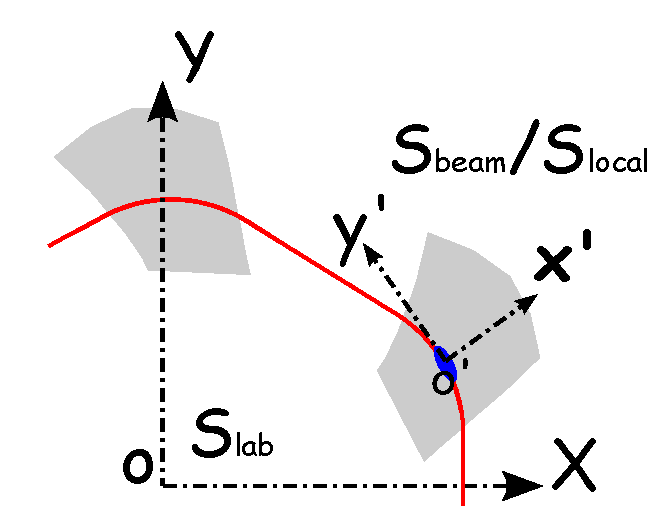
\includegraphics[width=5cm]{figures/SM-frame.pdf}
    \end{column}
  \end{columns}
  \begin{block}{3 frames defined}
    \begin{itemize}
    \item  ${\bs{S}_{\RM{lab}}}$  :  The global lab frame
    \item  ${\bs{S}_{\RM{local}}}$:  The local instantaneous frame
    \item  ${\bs{S}_{\RM{beam}}}$ :  The beam rest frame
    \end{itemize}
  \end{block}
}

\frame{
  \frametitle{3D Parallel Poisson Solver: \small{ P-M/FFT methods}}
  \begin{columns}
    \begin{column}{6.0cm}
      \begin{block}{}
        Space charge fields can be obtain by solving 
        the Poisson equation using Particle-Mesh (P-M) methods.
      \end{block}
    \end{column}
    \begin{column}{4.0cm}
      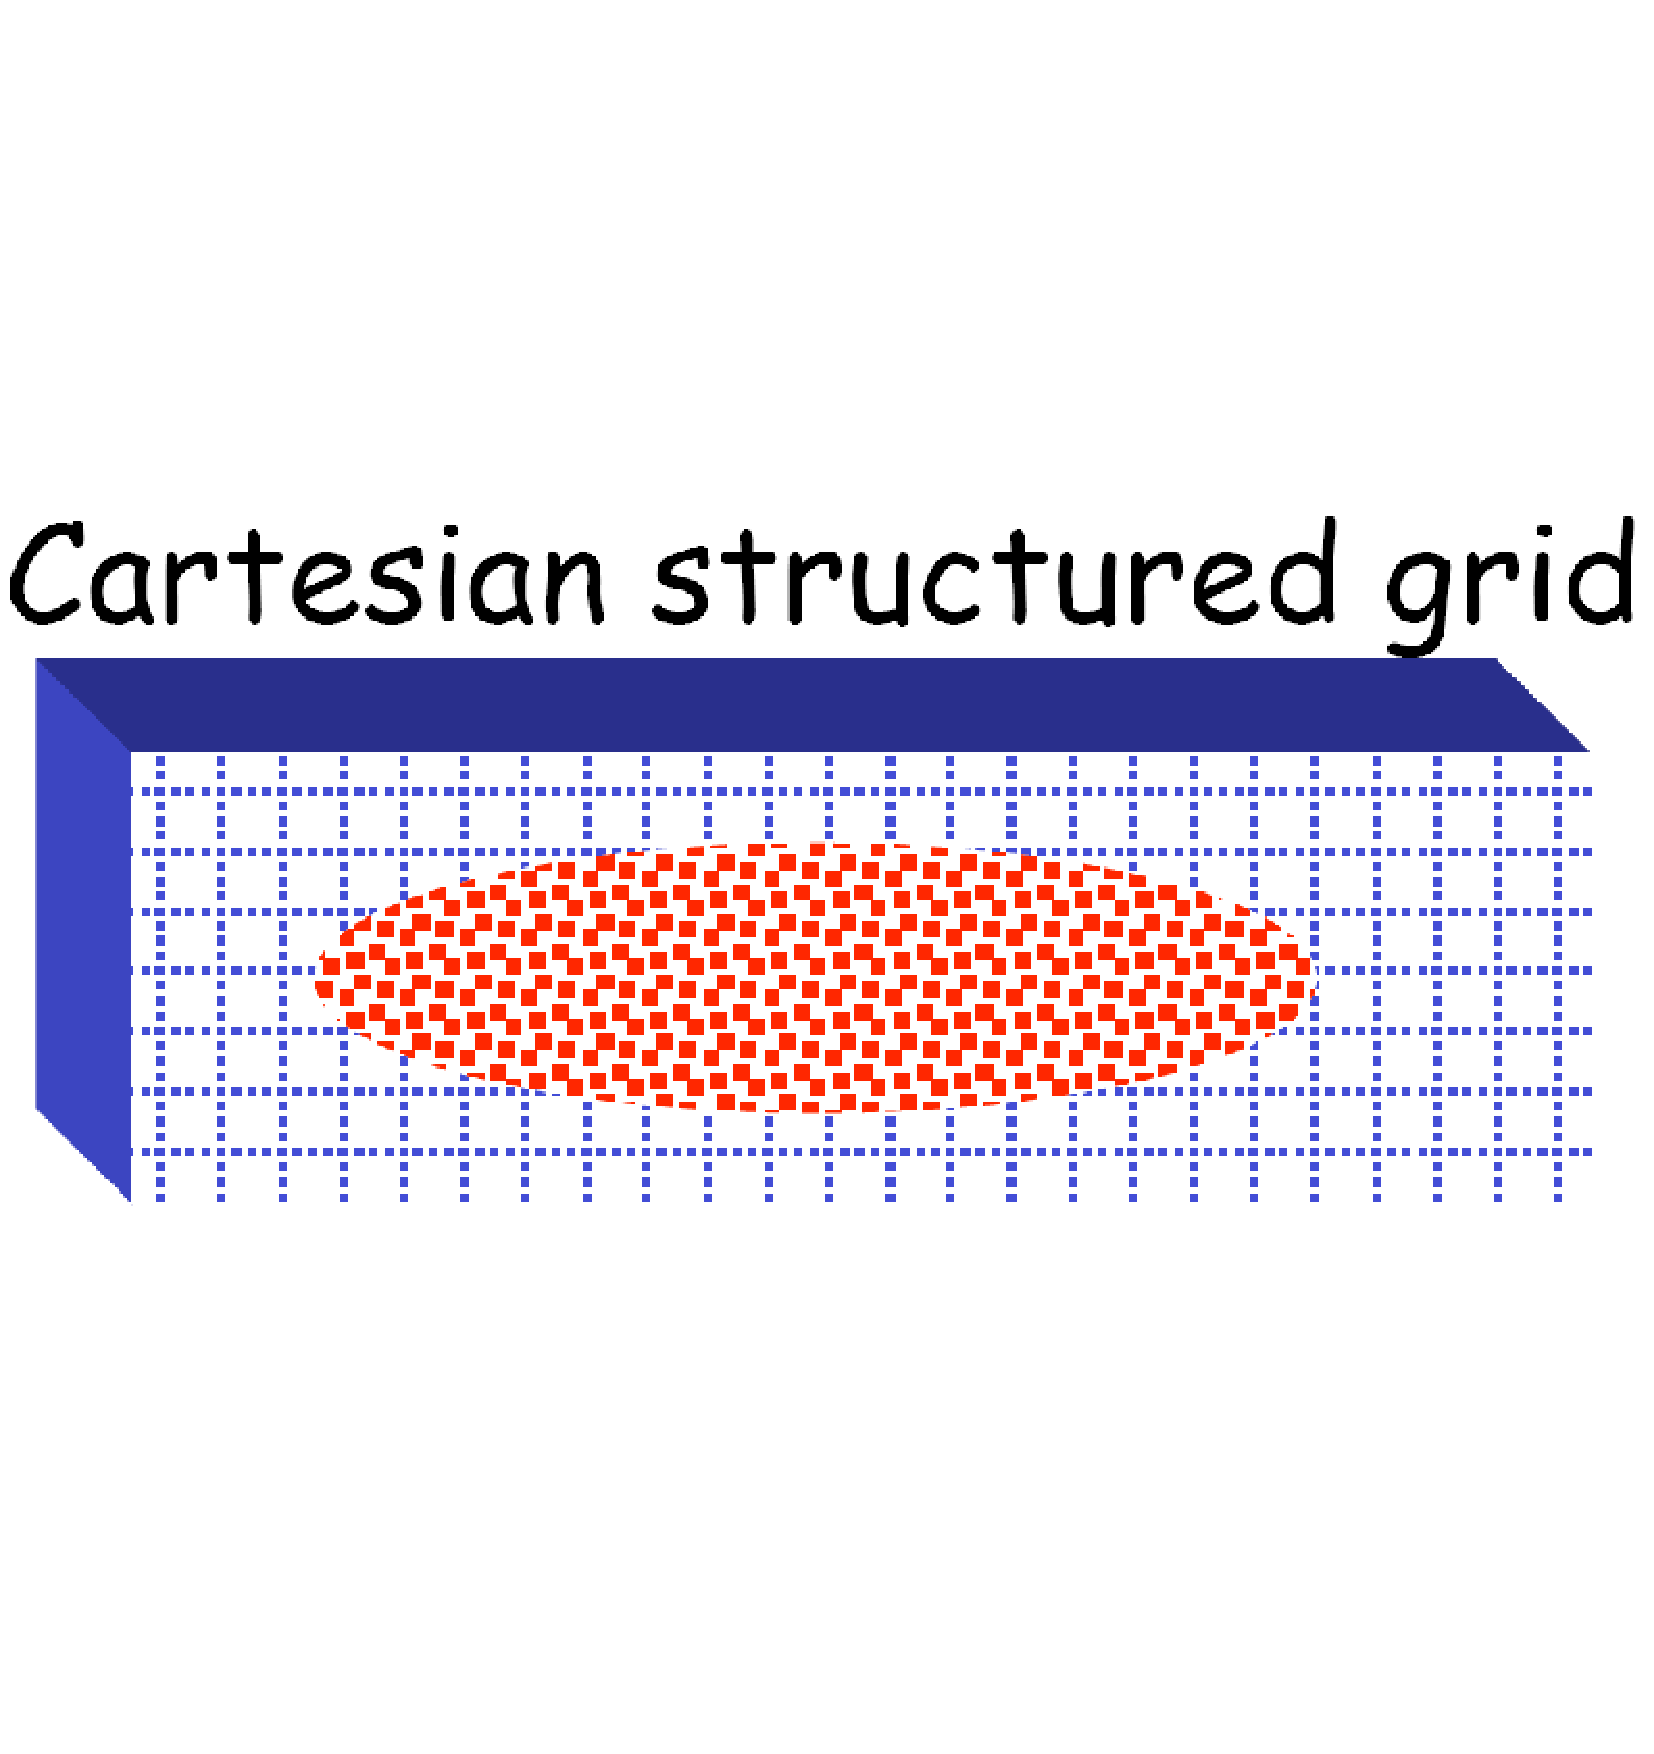
\includegraphics[width=4.0cm]{figures-slides/Grid}
    \end{column}
  \end{columns}

  \begin{block} {Solve Poisson equation on a rectangular domain with open BC }  
    A 3D rectangular grid which contains all particles is built (following quantities with superscript of $D$ means on grid).    
    The solution of the discretized Poisson equation with $\vec{k}=(l,n,m,)$
    \begin{equation*}\label{eq:DiscretizedPoisson}
      \nabla^{2} \phi^D(\vec{k}) = - \frac{\rho^D(\vec{k})}{\epsilon_0}, \vec{k} \in \Omega^D
    \end{equation*}
    
    $\phi^D$ is given by convolution with the appropriate discretized Green's function $G_D$: 
    \begin{equation*}
      \phi^D = \rho^D * G^D
    \end{equation*}
 %   Open or periodic boundary conditions can be applied.
  \end{block}

}

\frame{
  \frametitle{3D Parallel Poisson Solver: \small{ P-M/FFT methods}}  
  \begin{block}{Typical Procedure of the Poisson Solver}
    \begin{tabbing}
      \quad $\triangleright$ Assign all particles charges $q_i$ to nearby mesh points to obtain $\rho^D$ \\
      \quad $\triangleright$ Lorentz transform to obtain $\rho^D$ in $\bs{S_{\RM{beam}}}$\\
      \quad $\triangleright$ Use FFT on $\rho^D$ and $G^D$ to obtain $\widehat{\rho}^D$ and $\widehat{G}^D$ \\
      \quad $\triangleright$ Determine $\widehat{\phi}^D$ on the grid using $\widehat{\phi}^D = \widehat{\rho}^D \cdot \widehat{G}^D$  \\
      \quad $\triangleright$ Use inverse FFT on $\widehat{\phi }^D$ to obtain $\phi^D$\\
      \quad $\triangleright$ Compute $\bs{E}^D= -\nabla \phi^D$\\
      \quad $\triangleright$ Interpolate $\bs{E}$ at particle positions $\bs{x}$ from $\bs{E}^D$ \\
      \quad $\triangleright$ Lorentz back transform to obtain $\bs{E_{\RM{sc}}}$ and $\bs{B_{\RM{sc}}}$ in $\bs{S_{\RM{lab}}}$\\ 
    \end{tabbing}
  \end{block}
  
}

\subsection{Modeling Neighboring bunch effects}
\frame{
  \frametitle{Neighboring Bunch Effects: \small{Multi-bunch model}}
  \begin{block}{Multi-bunch model}
    In our model, the injection-to-extraction simulation is divided into two stages,  
    \begin{itemize}
    \item First stage, big $\Delta R$  \alert{$\Rightarrow$}  single bunch tracking
    \item Second stage, small $\Delta R$ \alert{$\Rightarrow$}  multiple bunches tracking
    \end{itemize} 
    The working mode transfers from single bunch mode to multiple bunches mode automatically when
    $\Delta R$ is comparable with the size of bunch.
  \end{block}

  \begin{block}{Summary}
    \begin{itemize}
    \item Fully self-consistent model of dealing with \rnb effects in time domain
    \item Using multiple bunches simulation, \nbe can be evaluated precisely
    \end{itemize} 
  \end{block}  
}

\frame{
  \frametitle{Neighboring Bunch Effects: \small{Algorithm}}
  \includegraphics[height=7cm]{figures-slides/NBplot.pdf}
}

\frame{
  \frametitle{Neighboring Bunch Effects: \small{Algorithm}}
  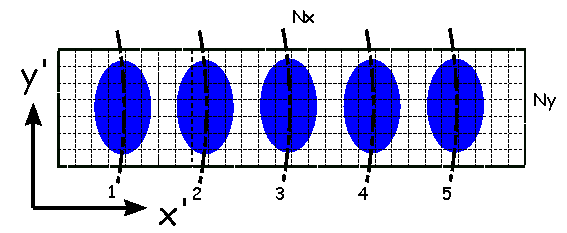
\includegraphics[width=8cm]{figures/SM-MultiBunch.pdf}
  \begin{block}{Energy bins}
    \begin{itemize}
    \item One energy bin for each bunch
    \item All particles grouped into bins
    \item Compute each bin's contribution separately
    \item Rebin when energy spread exceeds a given threshold value
    \end{itemize}
  \end{block}
}

\section{Validations and Applications}

\subsection{\opalcycl Scaling }

\begin{frame} 
  \frametitle{Parallel Scalability: \small{Test on Cray XT3 at CSCS, Switzerland}}
  \begin{columns}
    \begin{column}{4.cm}
      \scriptsize
      \begin{block}{Setup}
        \begin{itemize}
        \item  \alert{$10^6$} particles, 
        \item 3D FFT on a  \alert{$64^3$} grid,
	\item \alert{2D} domain decomposition
	\item Track  \alert{200} time steps
        \item Gaussian distribution
	\item Dump data into \alert{single} H5Part file every 10 steps
        \end{itemize}
      \end{block}
      
      \begin{block}{Observations}
        \begin{itemize}
        \item The code scales well
	\item Good load-balancing
	\item Dumping time increased 
        \end{itemize}
      \end{block}
    \end{column}
    \begin{column}{6.5cm}
    \begin{block}{}    
      \includegraphics[width=\linewidth]{figures/Timing64mesh}
      \center Time to solution is reduced approximately by a factor of \alert{60}, (256P Vs 1P).
    \end{block}  
    \end{column}
  \end{columns}
\end{frame}

\subsection{Applications}

\frame{
  \frametitle{Application I: \small{PSI 590MeV Ring}}
  \framesubtitle{Accelerating orbit and tune diagram}
  \begin{block}{}
  \begin{columns}
    \begin{column}{5.0cm}
      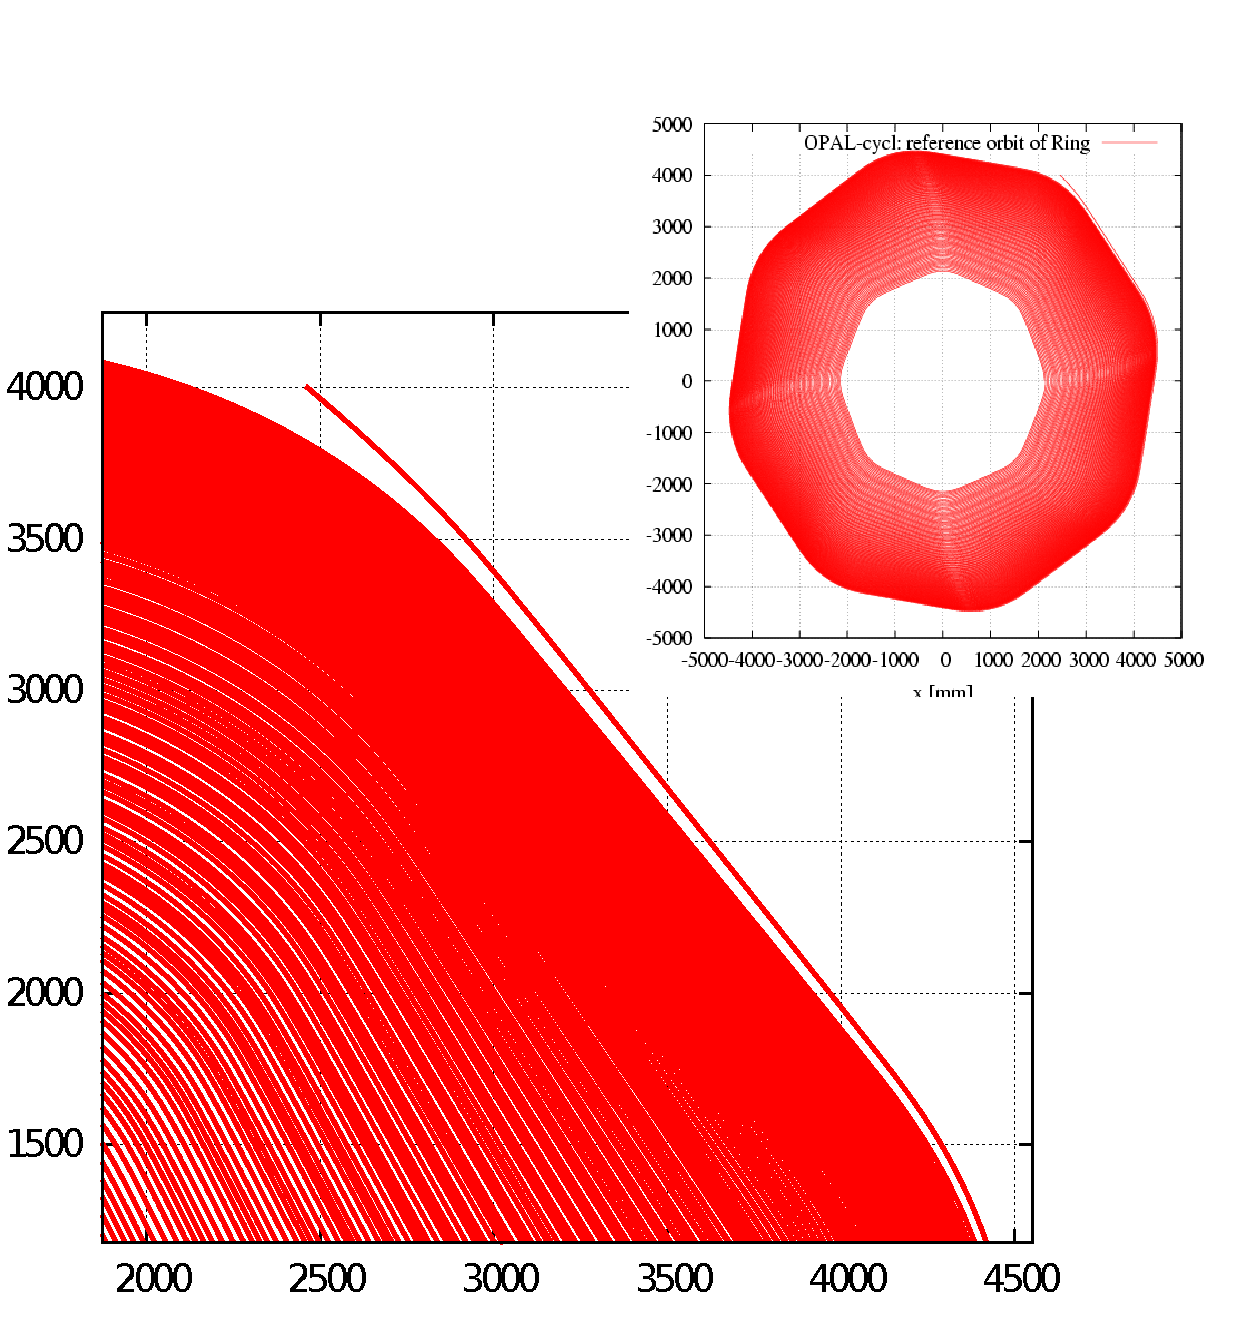
\includegraphics[width=\linewidth]{figures-slides/AEO-Ring2.pdf}         
    \end{column}
    \begin{column}{5.0cm}
      \includegraphics[width=\linewidth]{figures-slides/nurnuz_Ring} \\
      Tune calculation result is agree with FIXPO code very well!
    \end{column}
  \end{columns}
  \end{block}
}

\frame{
  \frametitle{Application I: \small{PSI 590MeV Ring}}
  \framesubtitle{\alert {Simulation} and \alert{measurement} }
  \begin{block}{}
  \begin{columns}
    \begin{column}{5.0cm}
      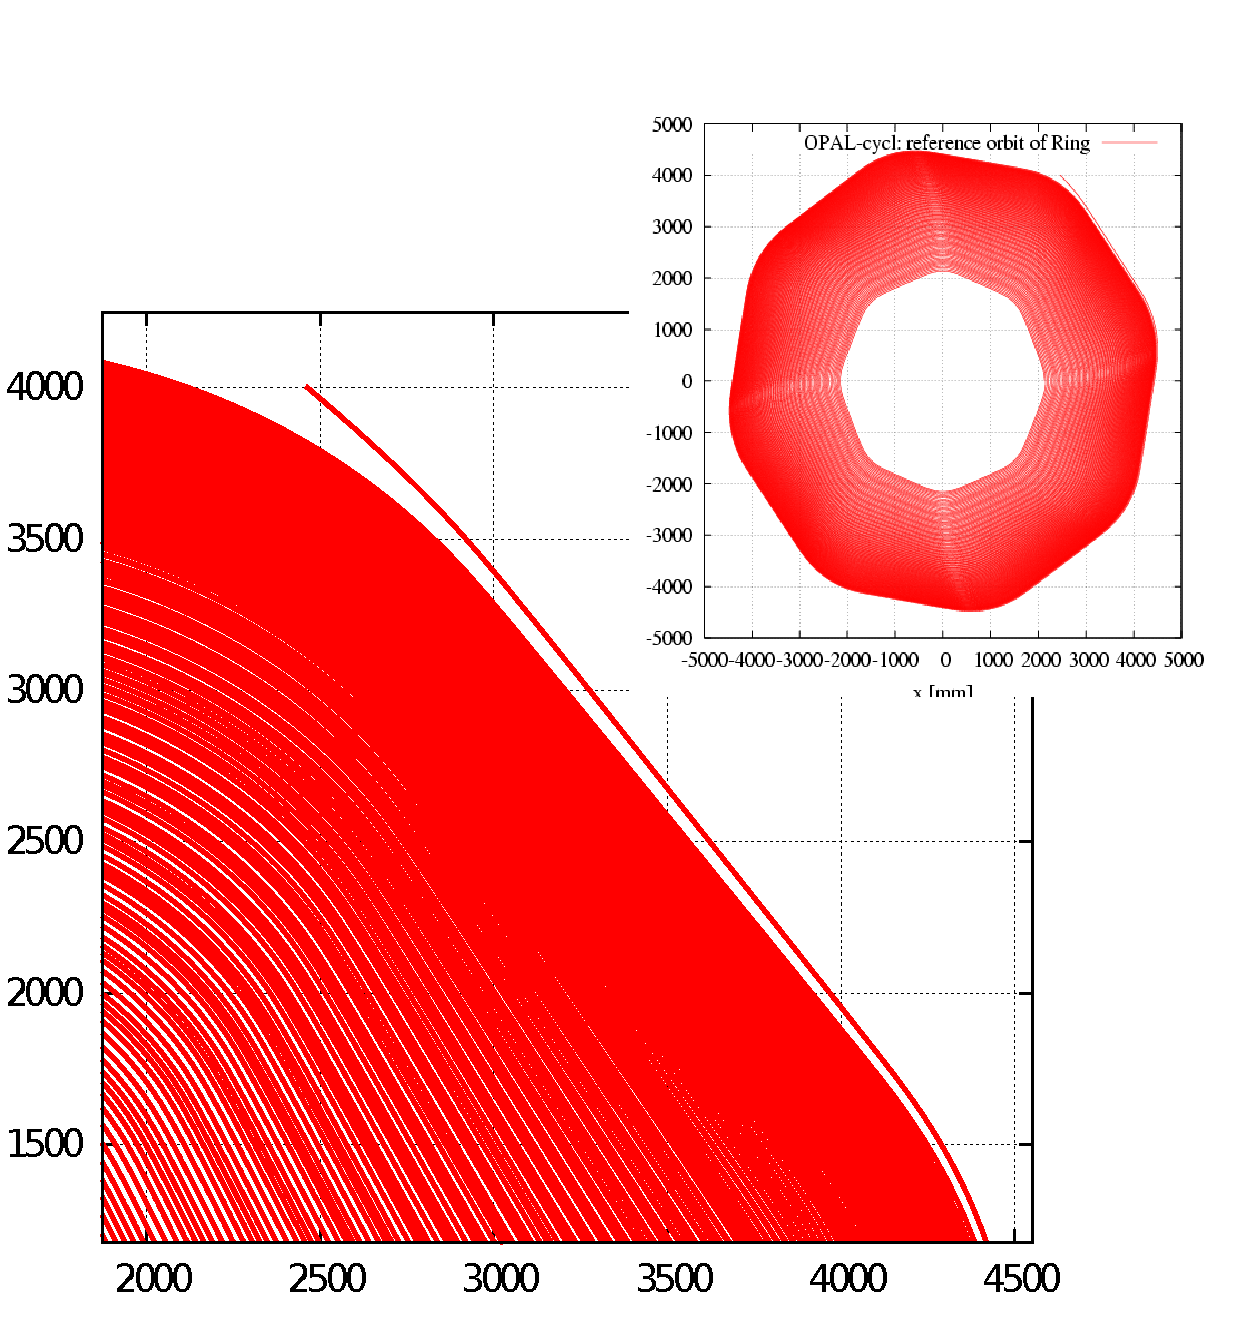
\includegraphics[width=\linewidth]{figures-slides/AEO-Ring2.pdf}
    \end{column}
    \begin{column}{5.0cm}
      \includegraphics[width=\linewidth]{figures-slides/measureNew1.pdf} \\
      Beam center position difference is less than +/- 5 mm.
    \end{column}
  \end{columns}
  \end{block}
}


\frame{
  \frametitle{Application I: \small{PSI 590MeV Ring}}
  \framesubtitle{\alert{Single bunch} with space charge}

  \begin{block}{Compare different initial phase widths of 3mA beam}  
  \begin{columns}
    \begin{column}{3.0cm}
      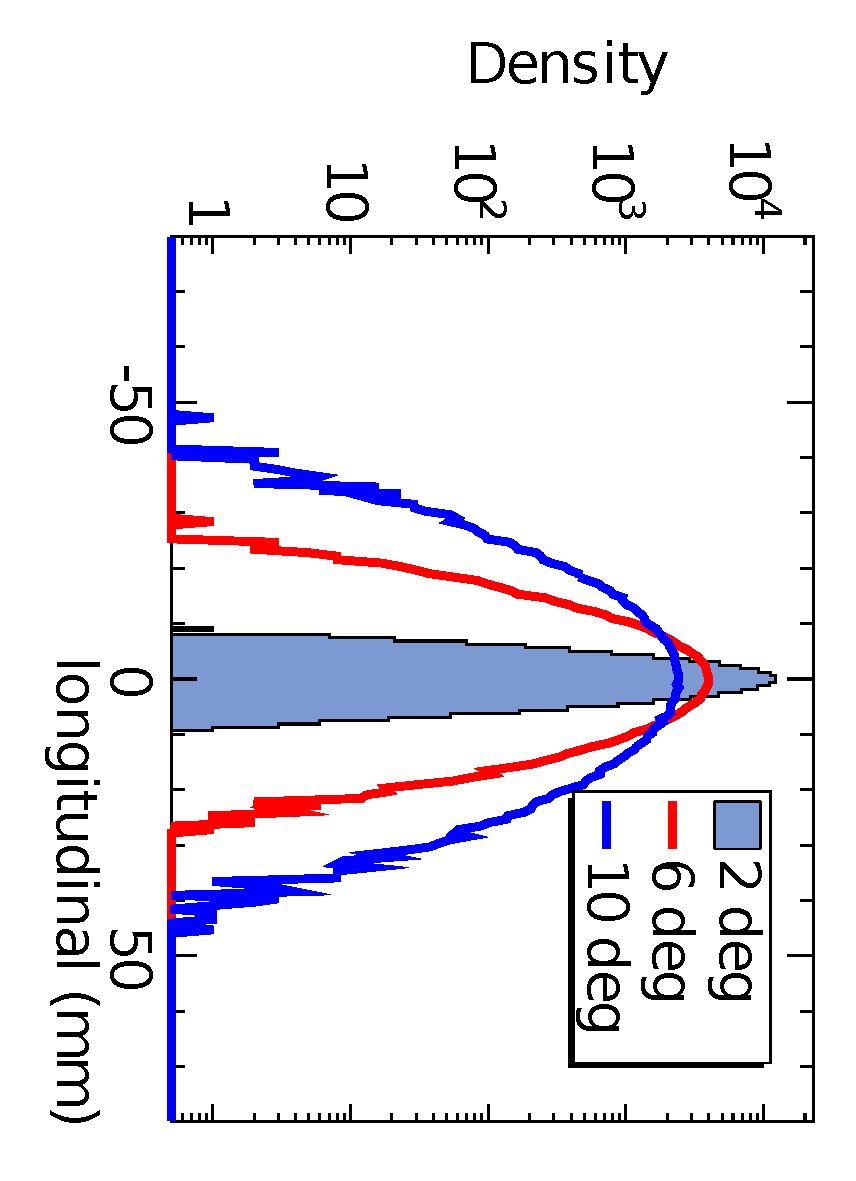
\includegraphics[angle=90,width=\linewidth]{figures/Theta-Turn-0.pdf} \\
      \center Turn 0
    \end{column}
    \begin{column}{3.0cm}
      \includegraphics[angle=90,width=\linewidth]{figures/Theta-Turn-50.pdf} \\
      \center Turn 50
    \end{column}
    \begin{column}{3.0cm}
      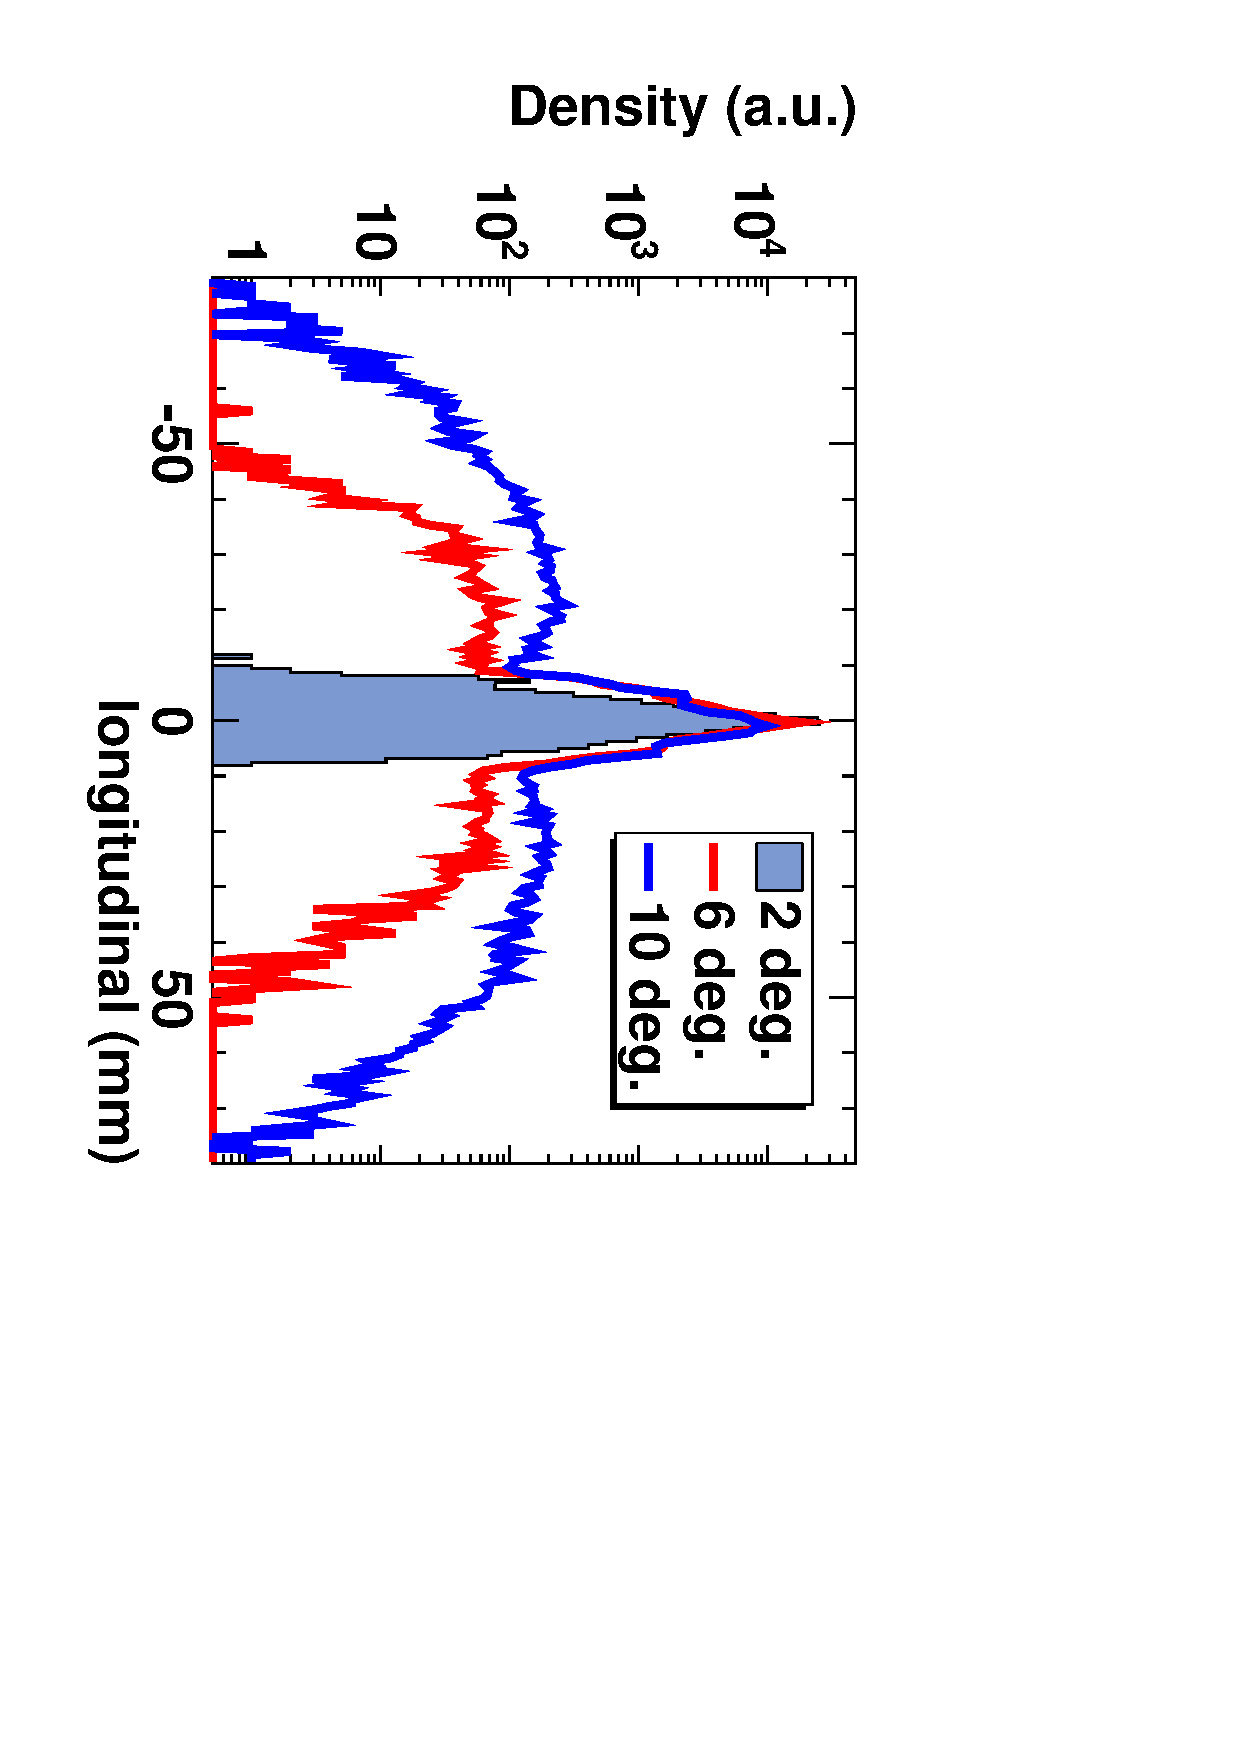
\includegraphics[angle=90,width=\linewidth]{figures/Theta-Turn-150.pdf} \\
      \center Turn 150
    \end{column}
  \end{columns}
  \end{block}
  \begin{block}{}  
    \begin{itemize}
      \item $2^o$:  Keep compact shape, no tails exist
      \item $6^o$:  With tails about 3 cm long
      \item $10^o$: With long tails of more than 6 cm long
    \end{itemize}
  \end{block}

}

\frame{
  \frametitle{Application I: \small{PSI 590MeV Ring}}
  \framesubtitle{\alert{Single bunch} with space charge}

  \begin{block}{Start-to-end RMS sizes comparison of 3MeV beam}  
    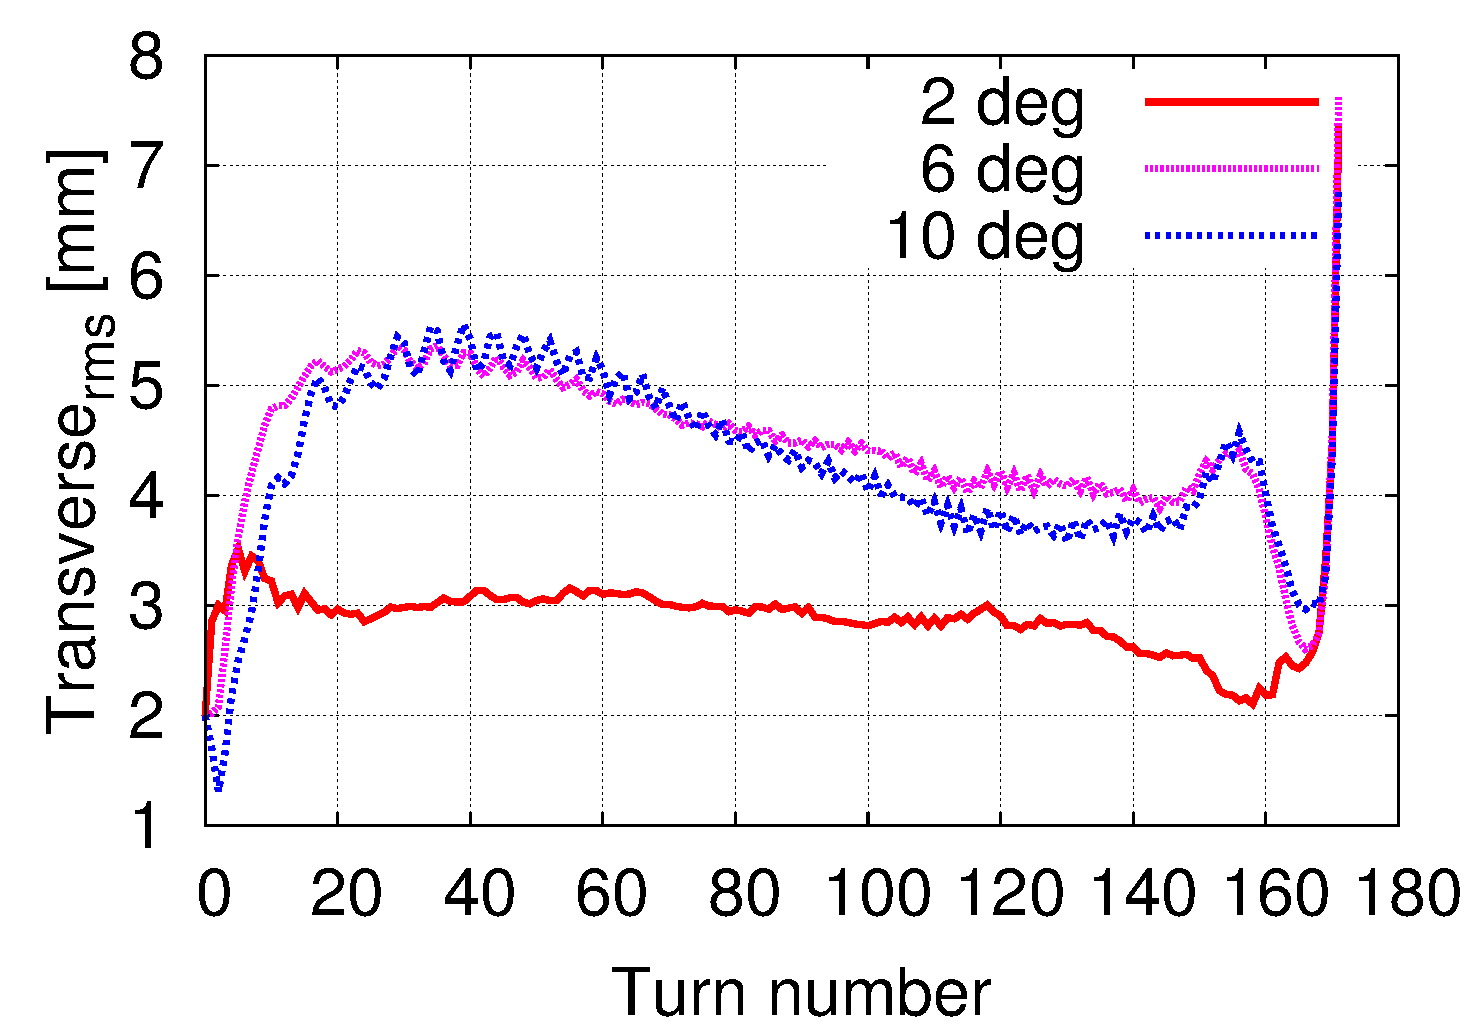
\includegraphics[width=0.48\linewidth]{figures/Comp-Transverse.pdf}
    \includegraphics[width=0.48\linewidth]{figures/Comp-Longitudinal.pdf}
  \end{block}
}

\frame{
  \frametitle{Application I: \small{PSI 590MeV Ring}}
  \framesubtitle{\alert{Single bunch}  and \alert{multiple bunches} at turn 80 and 130}
  
  \includegraphics[angle=90,width=0.95\linewidth]{figures/C9B7BSB-2D-1mA-80.pdf}\\
  \includegraphics[angle=90,width=0.95\linewidth]{figures/C9B7BSB-2D-1mA-130.pdf}
}


\frame{
 \frametitle{Application I: \small{PSI 590MeV Ring}}
  \framesubtitle{\alert{Single bunch}  and \alert{multiple bunches} at turn 80 and 130}
 
  \includegraphics[angle=90,width=0.42\linewidth]{figures/C9B7BSB-R-1mA-80.pdf}
  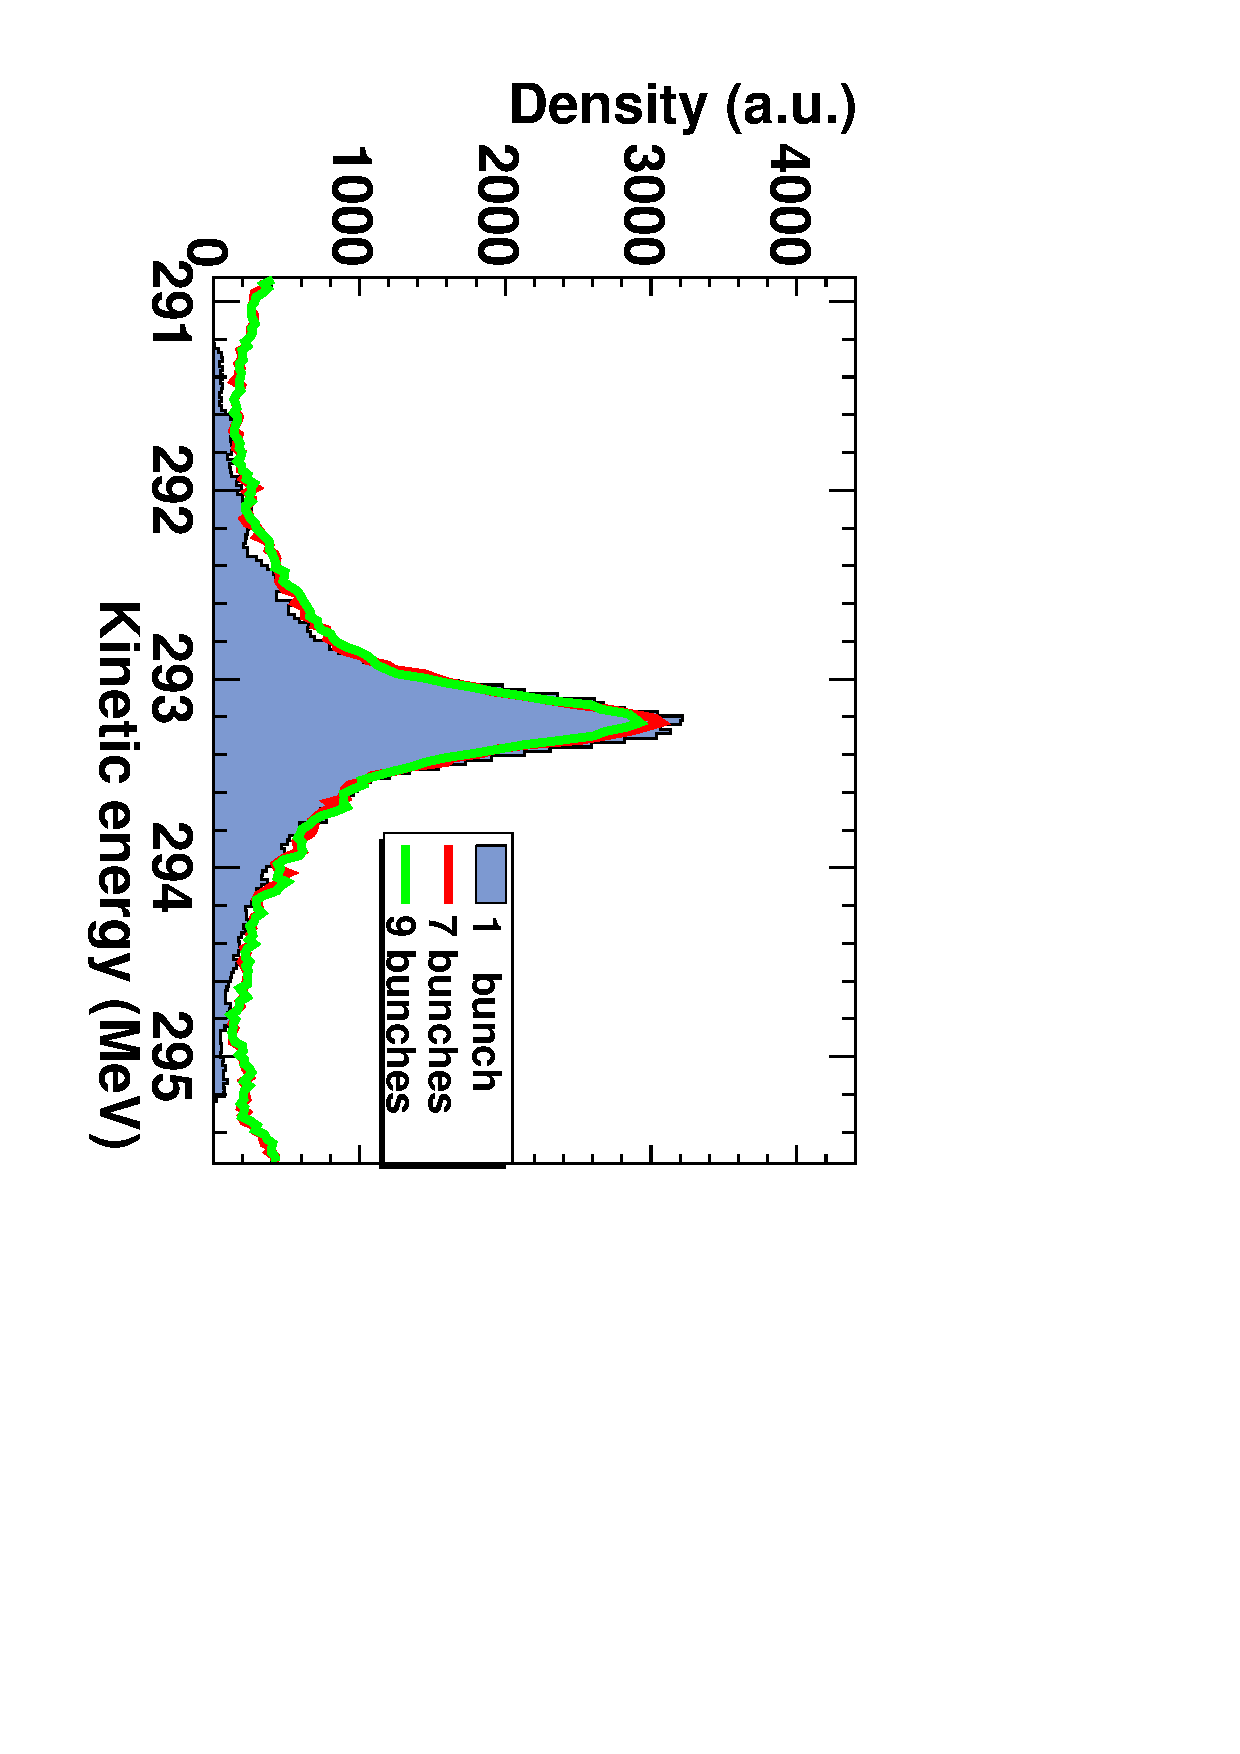
\includegraphics[angle=90,width=0.42\linewidth]{figures/C9B7BSB-Energy-1mA-80.pdf}\\
   \includegraphics[angle=90,width=0.42\linewidth]{figures/C9B7BSB-R-1mA-130.pdf}
  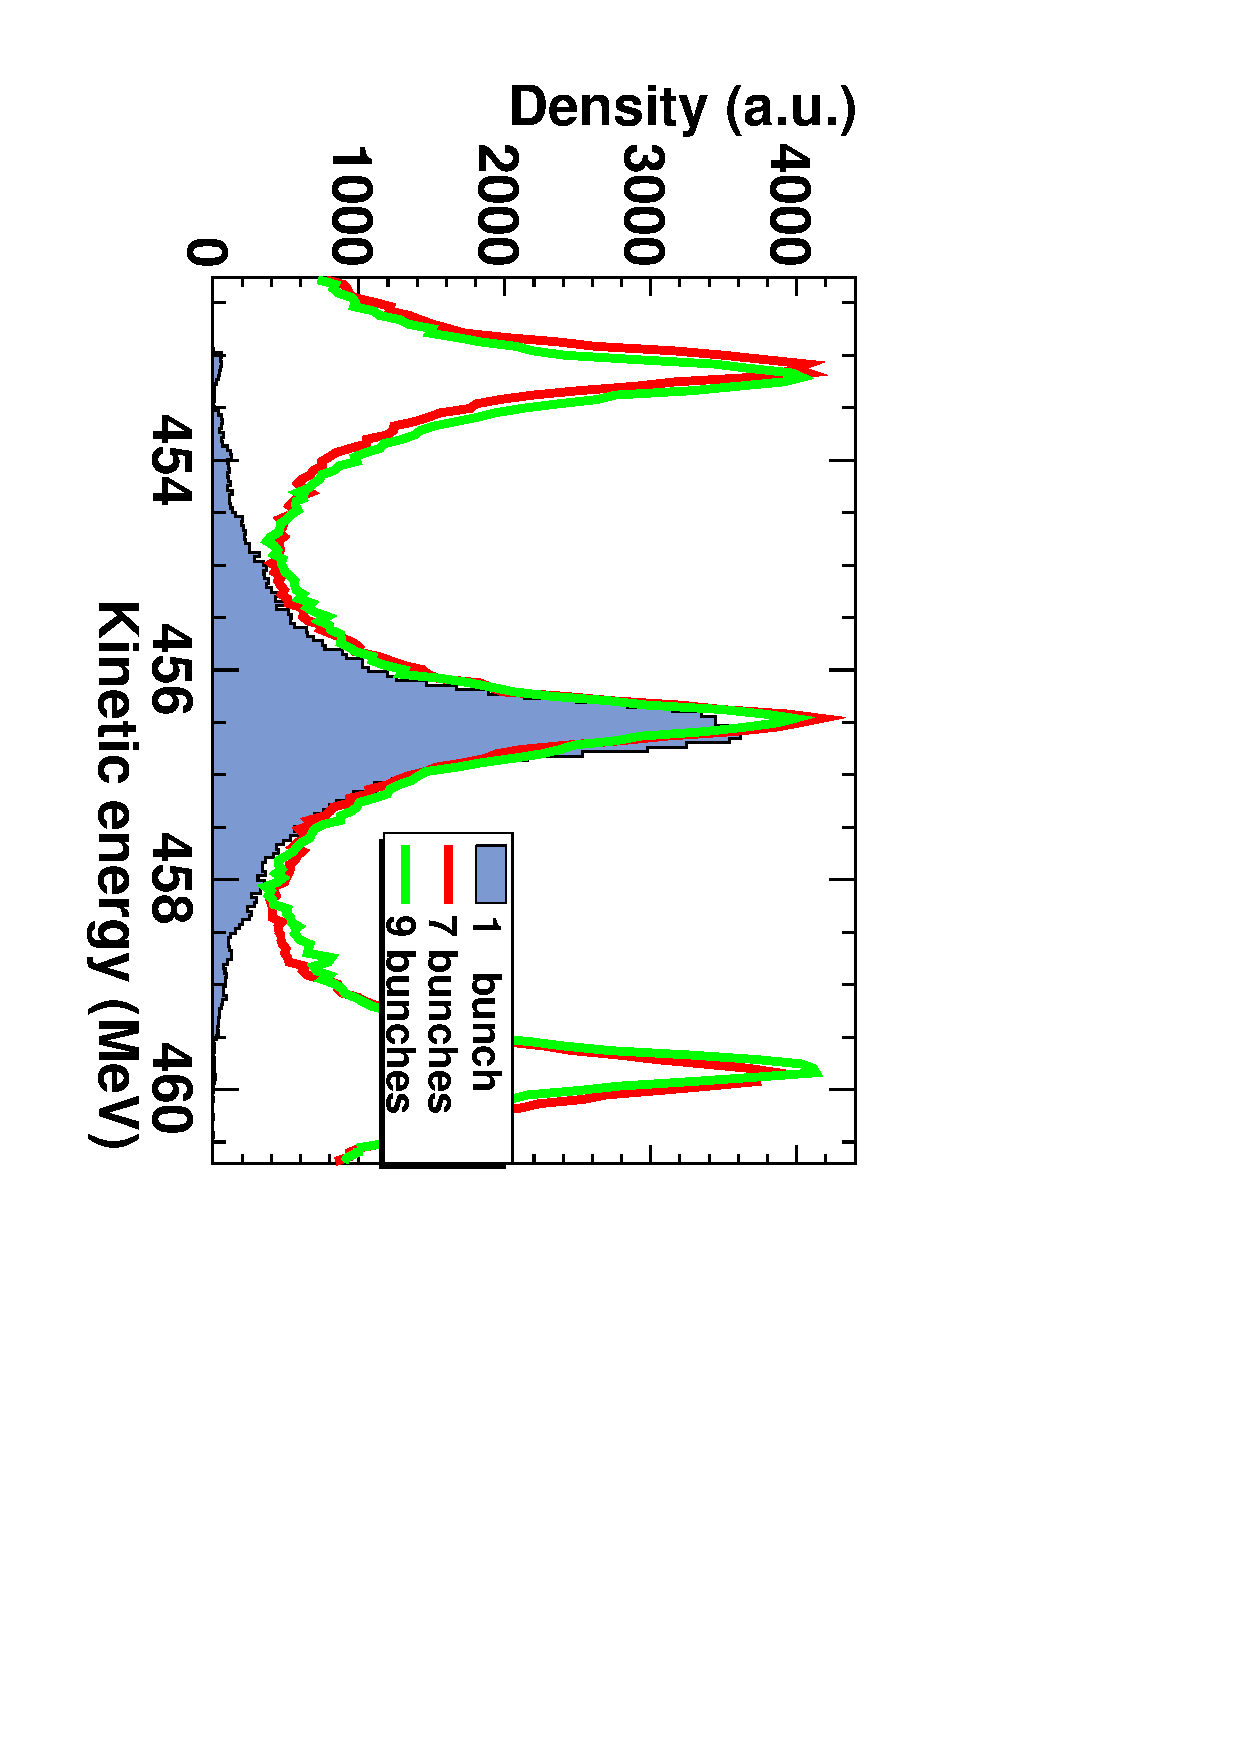
\includegraphics[angle=90,width=0.42\linewidth]{figures/C9B7BSB-Energy-1mA-130.pdf}
}

\frame{
  %url base
  \hyperbaseurl{/home2/yang/svnwork/OPAL/opal-Doc/doc/OPAL/presentations/HB08/}

  \frametitle{Application I: \small{PSI 590MeV Ring}}
  \framesubtitle{\alert{Single bunch}  and \alert{multiple bunches} at turn 80 and 130}
  
  \begin{block}{Animation movie}
  \center{\color{blue} \underline{\href{Movie/Ring9B3mA.mpeg} {Animation for 9 bunches injection and tracking}}}
  \\
  \end{block}

  \begin{block}{Conclusion of neighboring bunch effects of 1mA beam}

    \begin{itemize}
      \item 9 bunches is enough to give out precise solution
      \item It has visible impacts on beam dynamics
      \item It makes the bunch more compact in transverse direction
      \end{itemize}
  \end{block}
}

\frame{ 

  \frametitle{Application II: \small{PSI Injector II}}
  \framesubtitle{\alert{3 MeV coasting beam}}
  \begin{columns}
    \begin{column}{4.0cm}
      Animations of Beam development in 40 turns:\\
      {\color{blue}\underline{\href{Movie/0mA.mpeg}{0mA beam animation}}}\\
      {\color{blue}\underline{\href{Movie/1mA.mpeg}{1mA beam animation}}} \\
      {\color{blue}\underline{\href{Movie/3mA.mpeg}{3mA beam animation}}}
    \end{column}
    
    \begin{column}{6.0cm}
      \includegraphics[width=0.8\linewidth]{figures-slides/INJII.png}
    \end{column}
  \end{columns}  

  \begin{block}{Conclusion} 
    In Injector2, \sce help to develop a very compact stable core in the first several turns for more than 1mA beam.
  \end{block}
}

\frame{
  \frametitle{Application II: \small{PSI Injector II}}
  \framesubtitle{\alert{3 MeV coasting beam}}
  \center{
    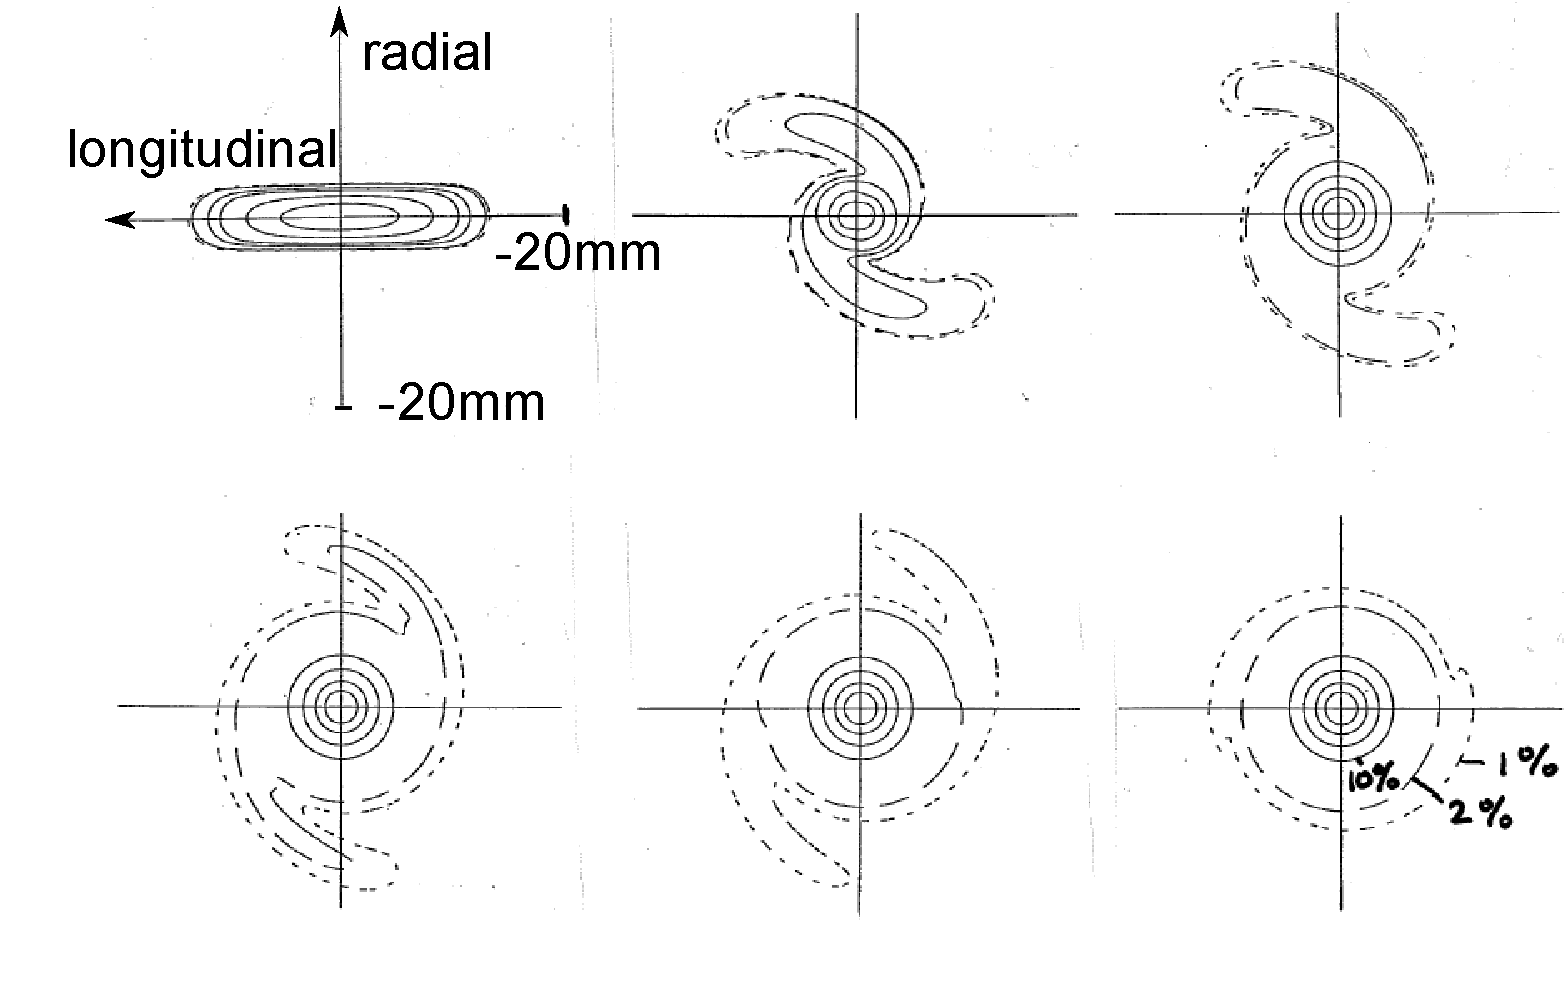
\includegraphics[width=0.8\linewidth]{figures-slides/PICS.pdf}\\
    I=1mA. Up: turn 0, 5, 10. Down: turn 20, 30, 40 by PICS (courtesy by S. Adam)
  }
}

\frame{
  \frametitle{Application II: \small{PSI Injector II}}
  \framesubtitle{\alert{3 MeV coasting beam}}
  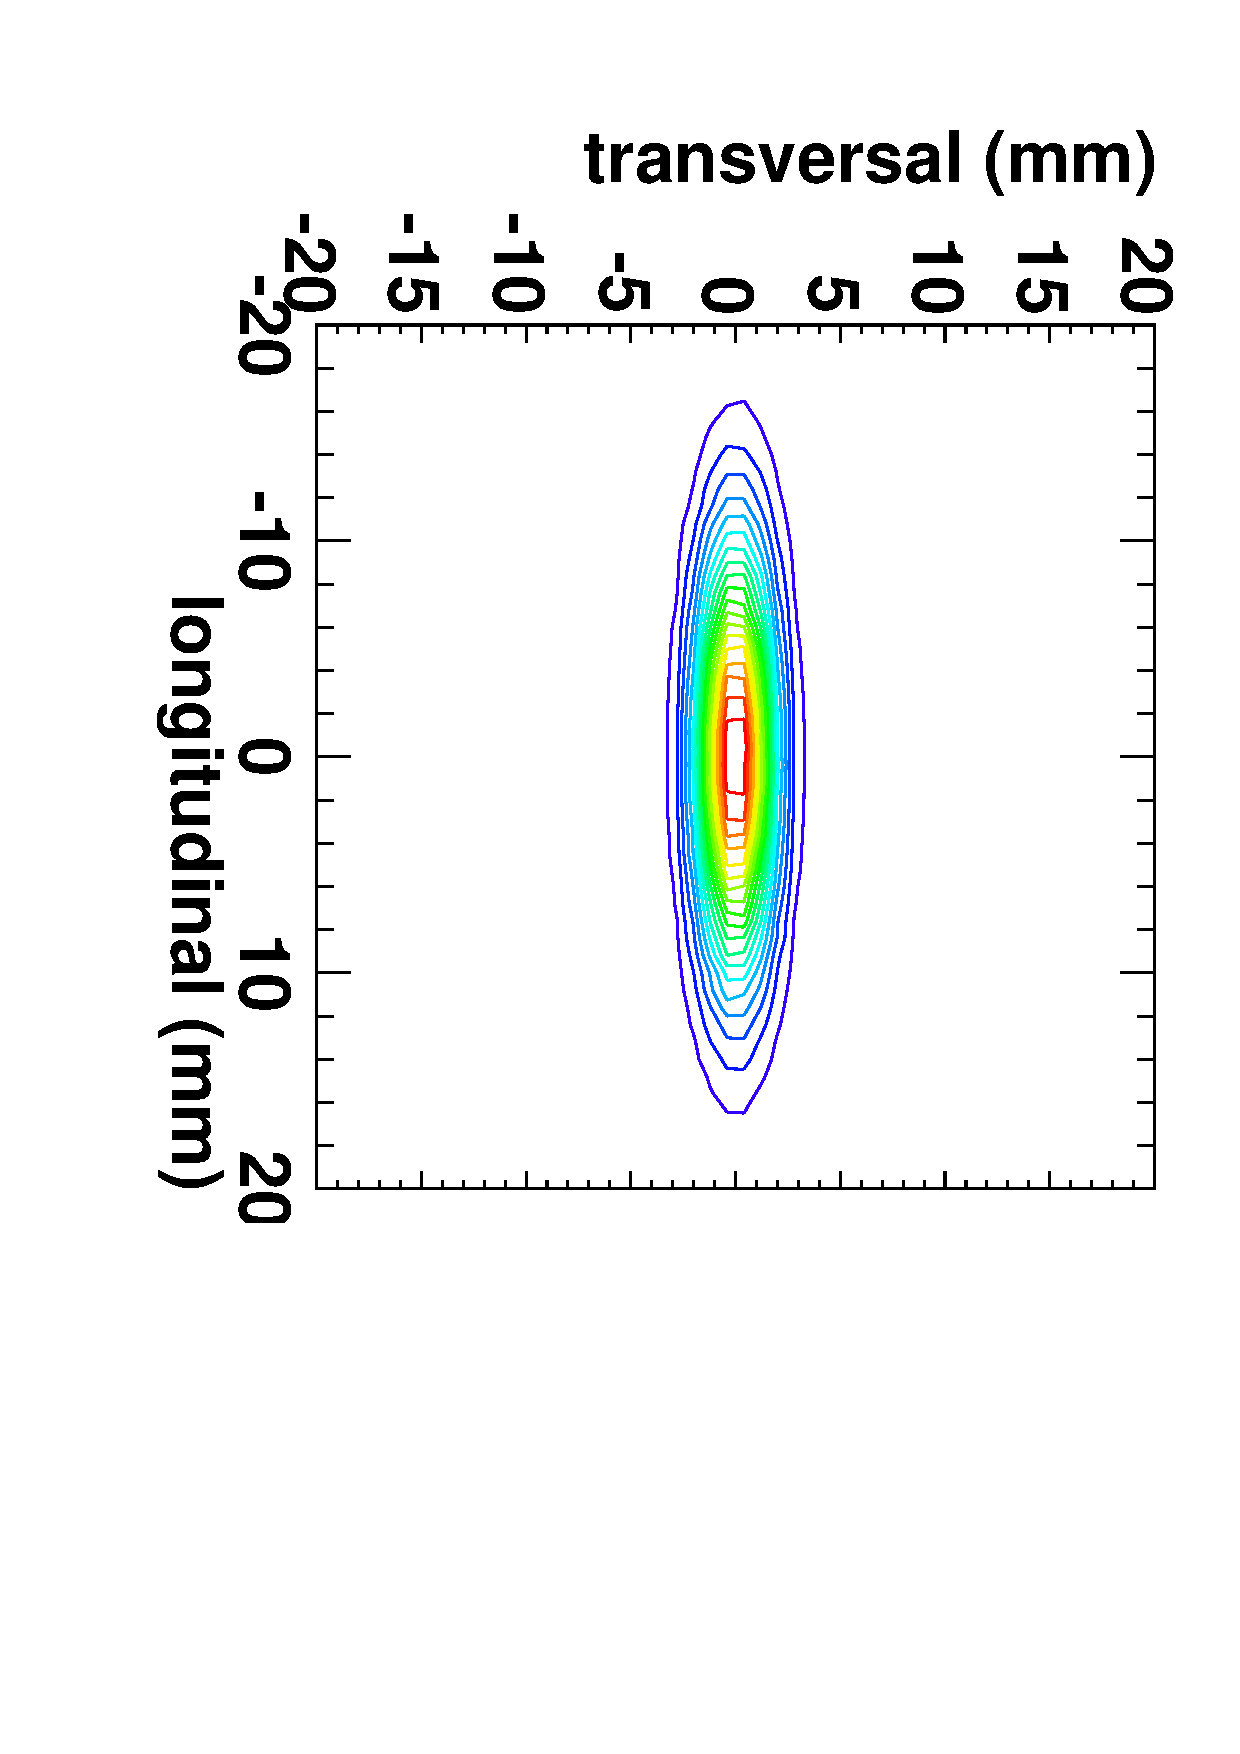
\includegraphics[angle=90,width=0.3\linewidth]{figures/Inj2/1mA0.pdf}
  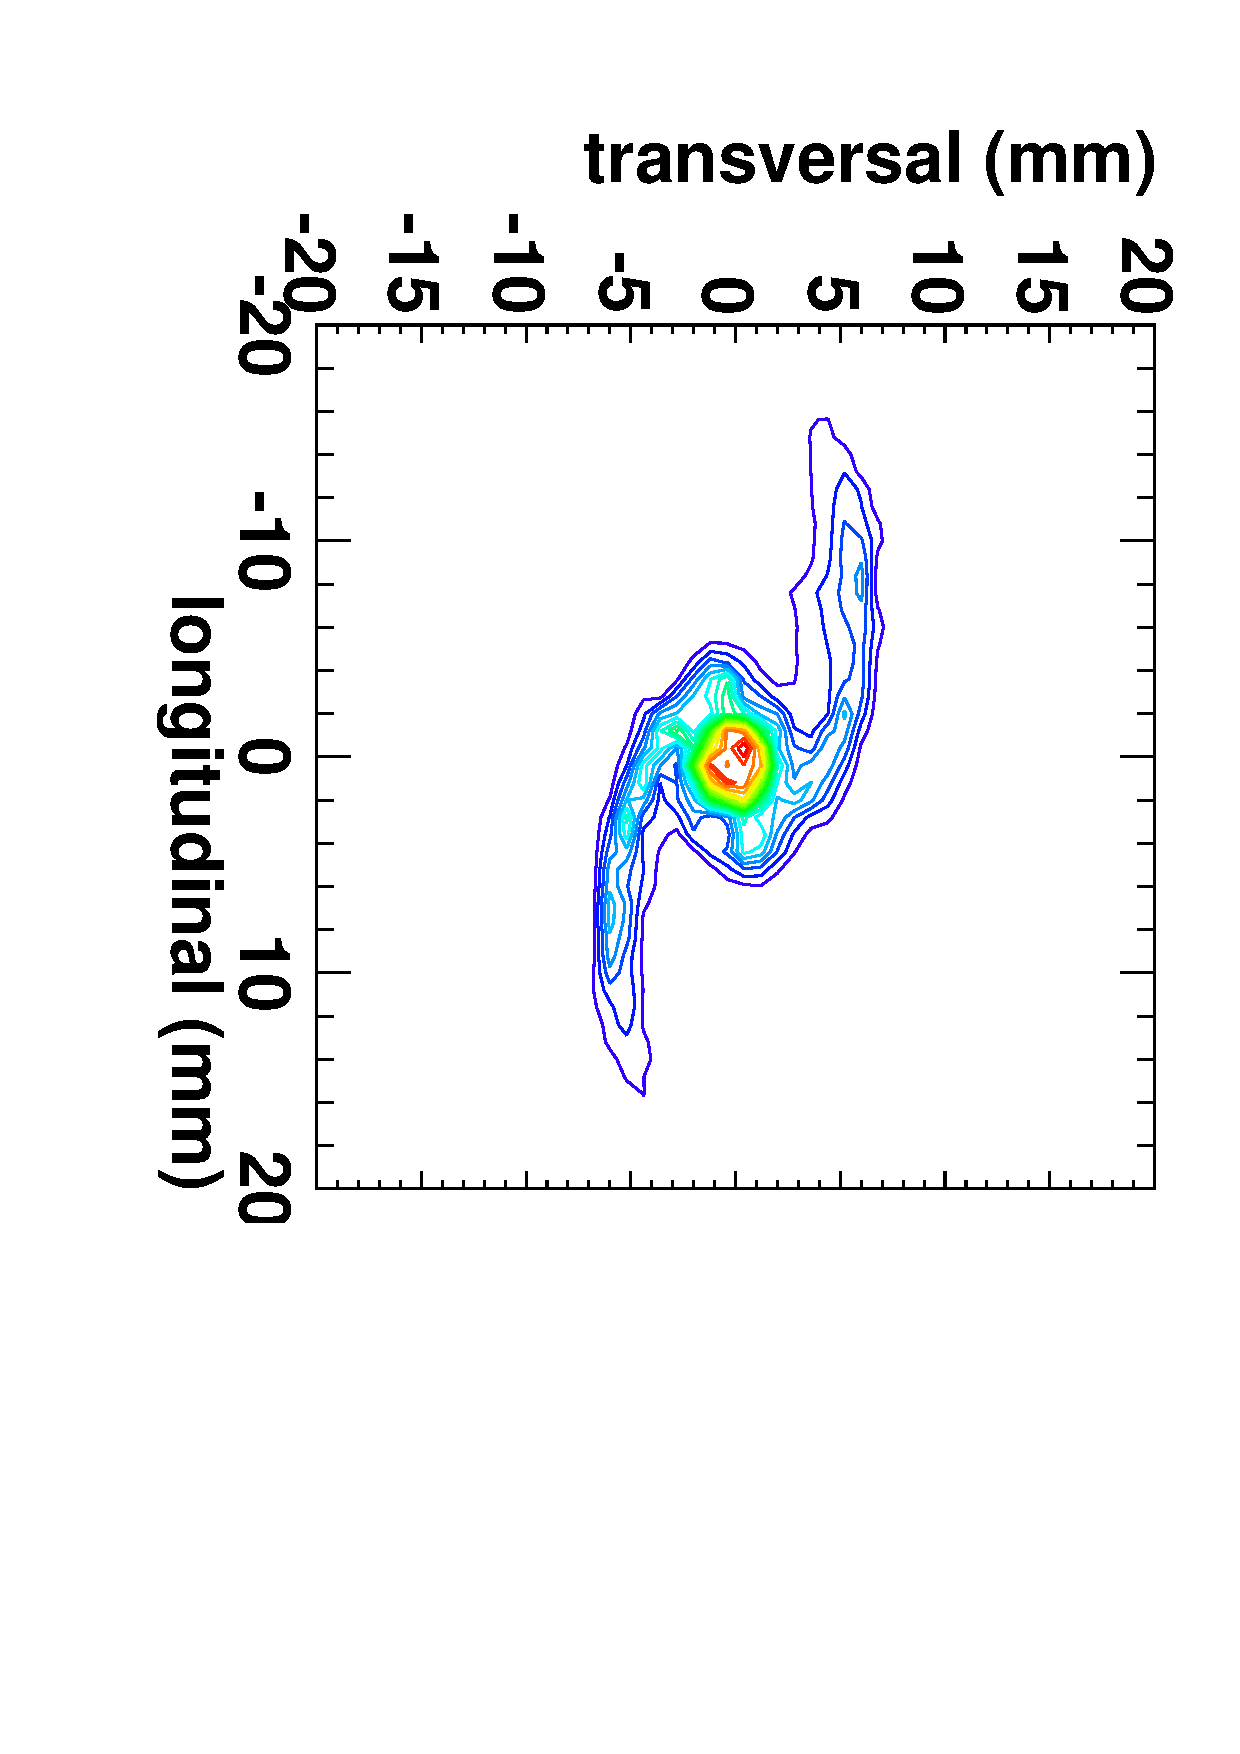
\includegraphics[angle=90,width=0.3\linewidth]{figures/Inj2/1mA5.pdf}
  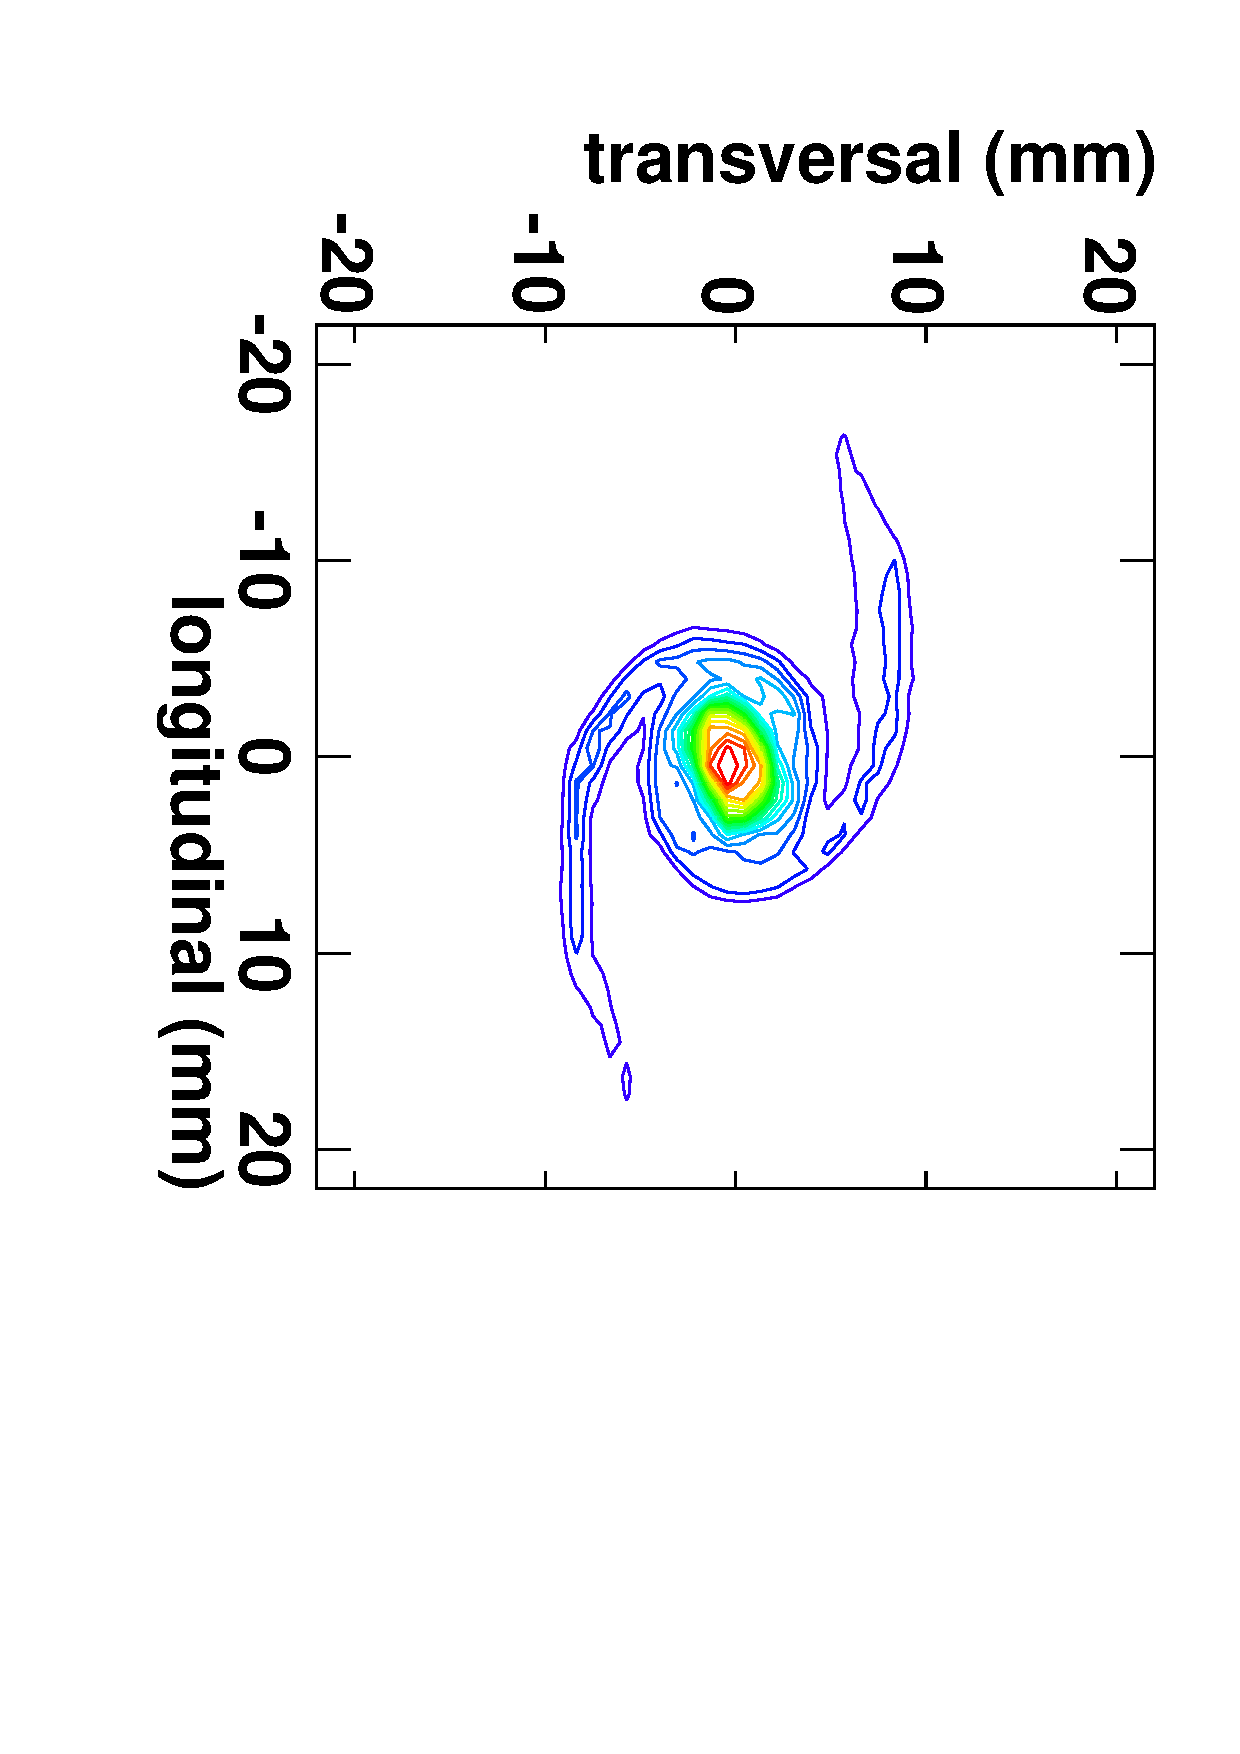
\includegraphics[angle=90,width=0.3\linewidth]{figures/Inj2/1mA10.pdf}\\
  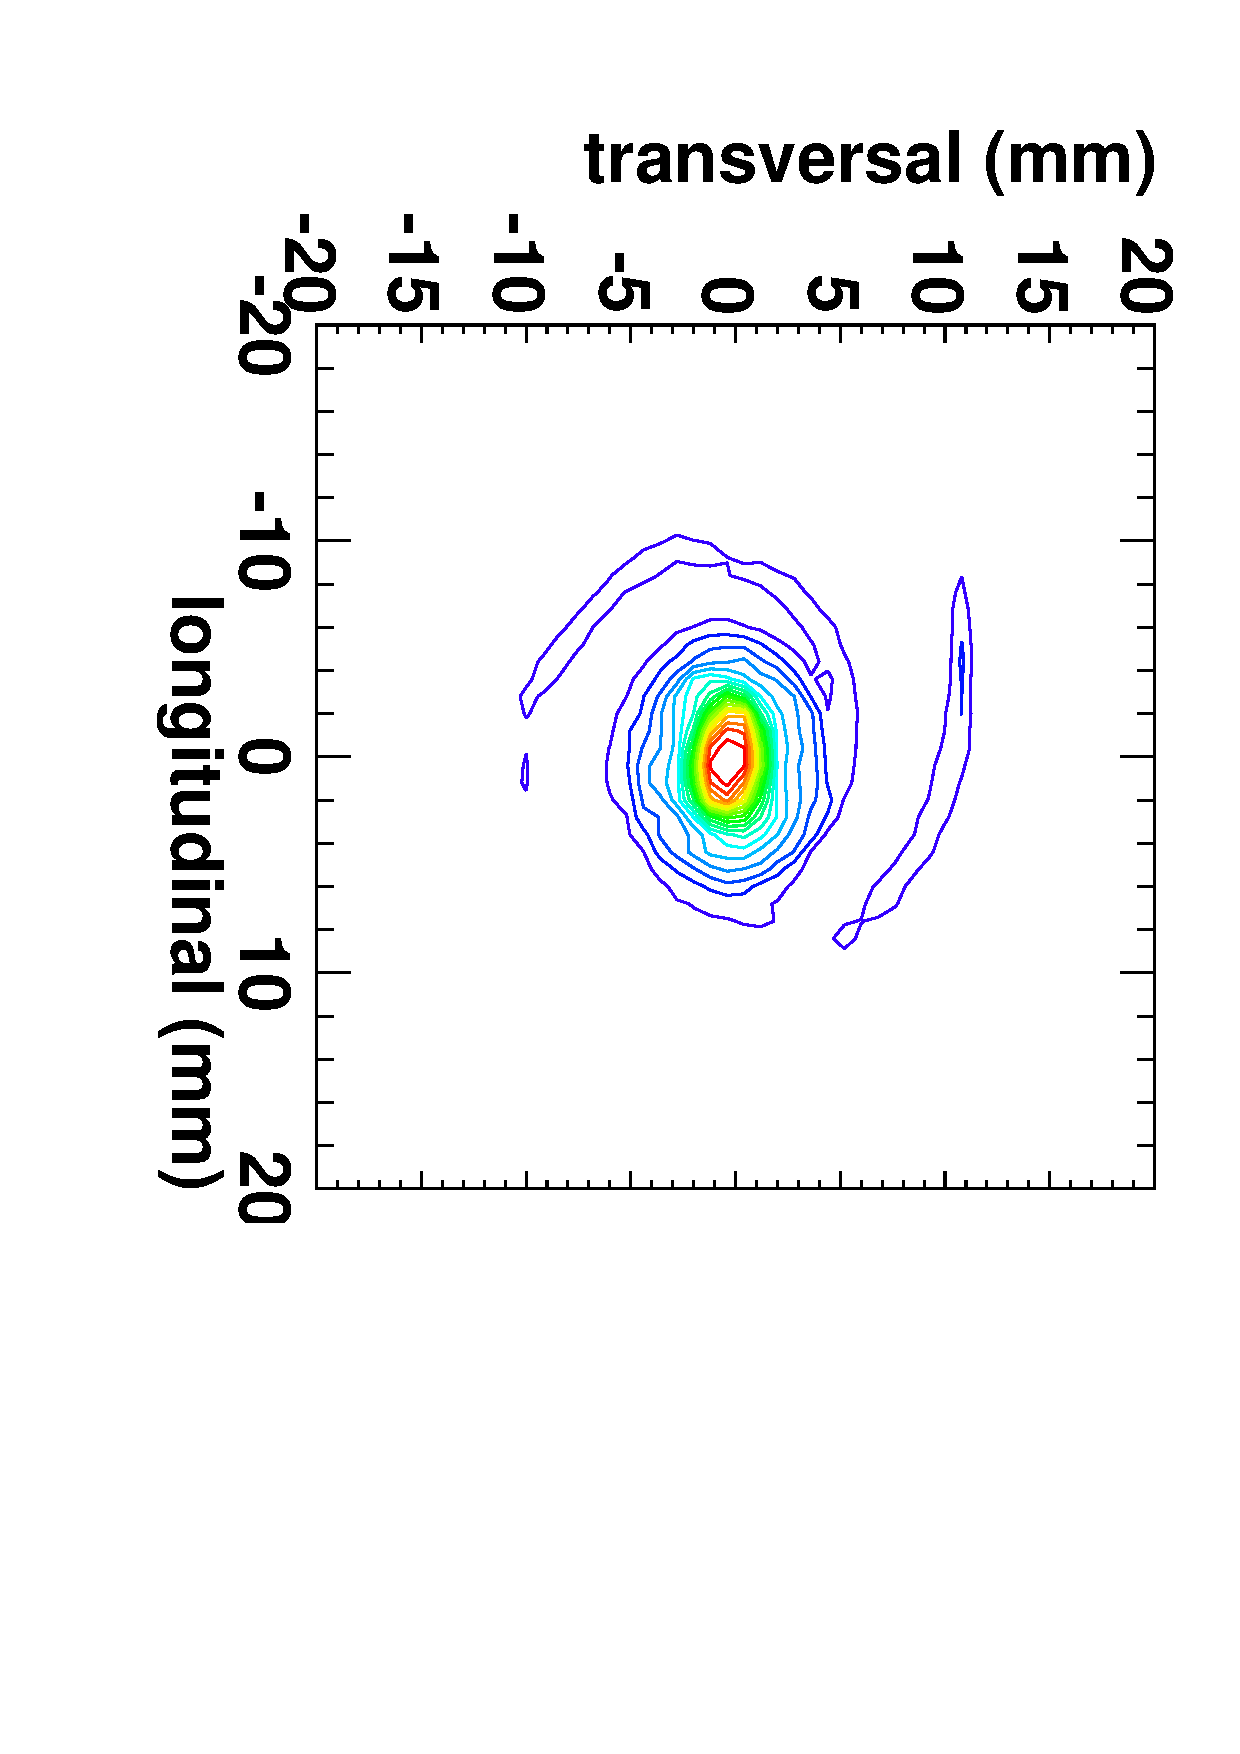
\includegraphics[angle=90,width=0.3\linewidth]{figures/Inj2/1mA20.pdf}
  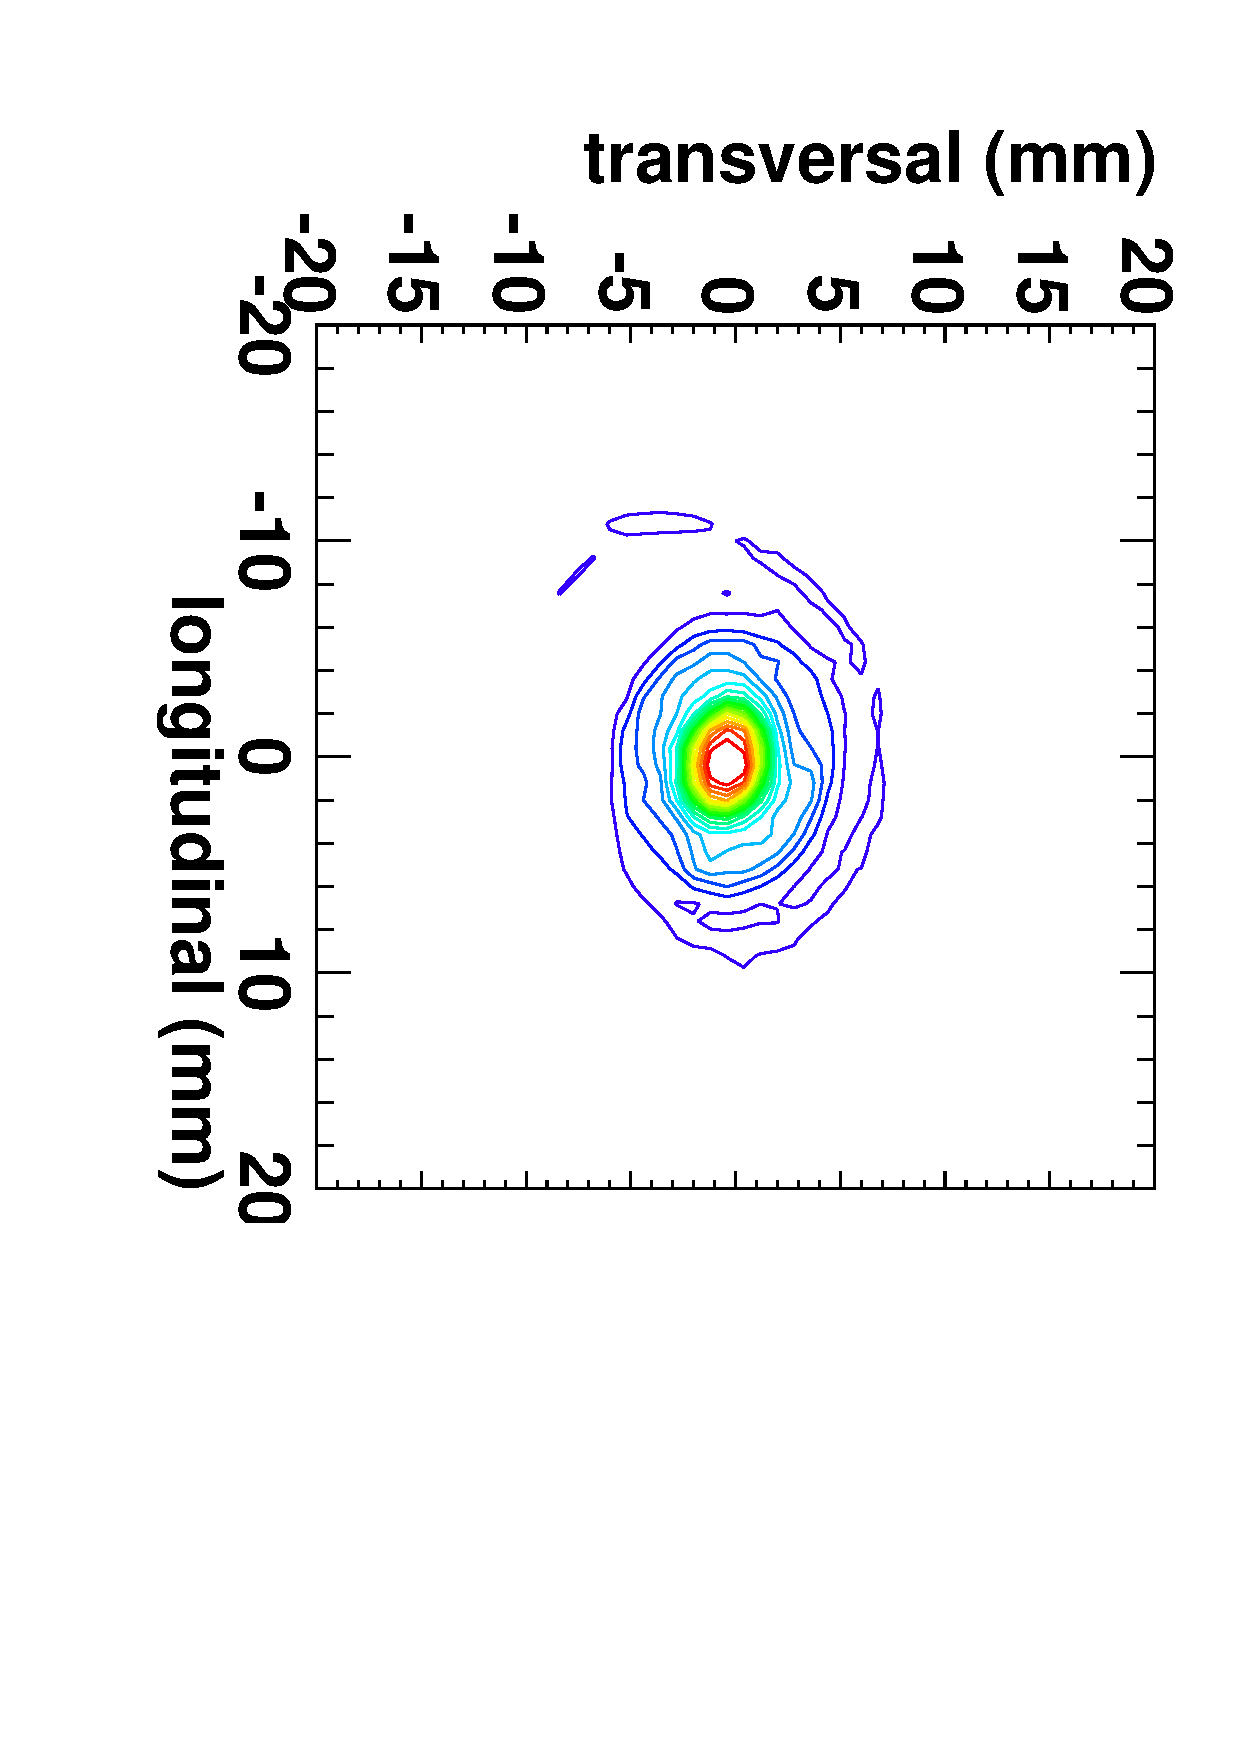
\includegraphics[angle=90,width=0.3\linewidth]{figures/Inj2/1mA30.pdf}
  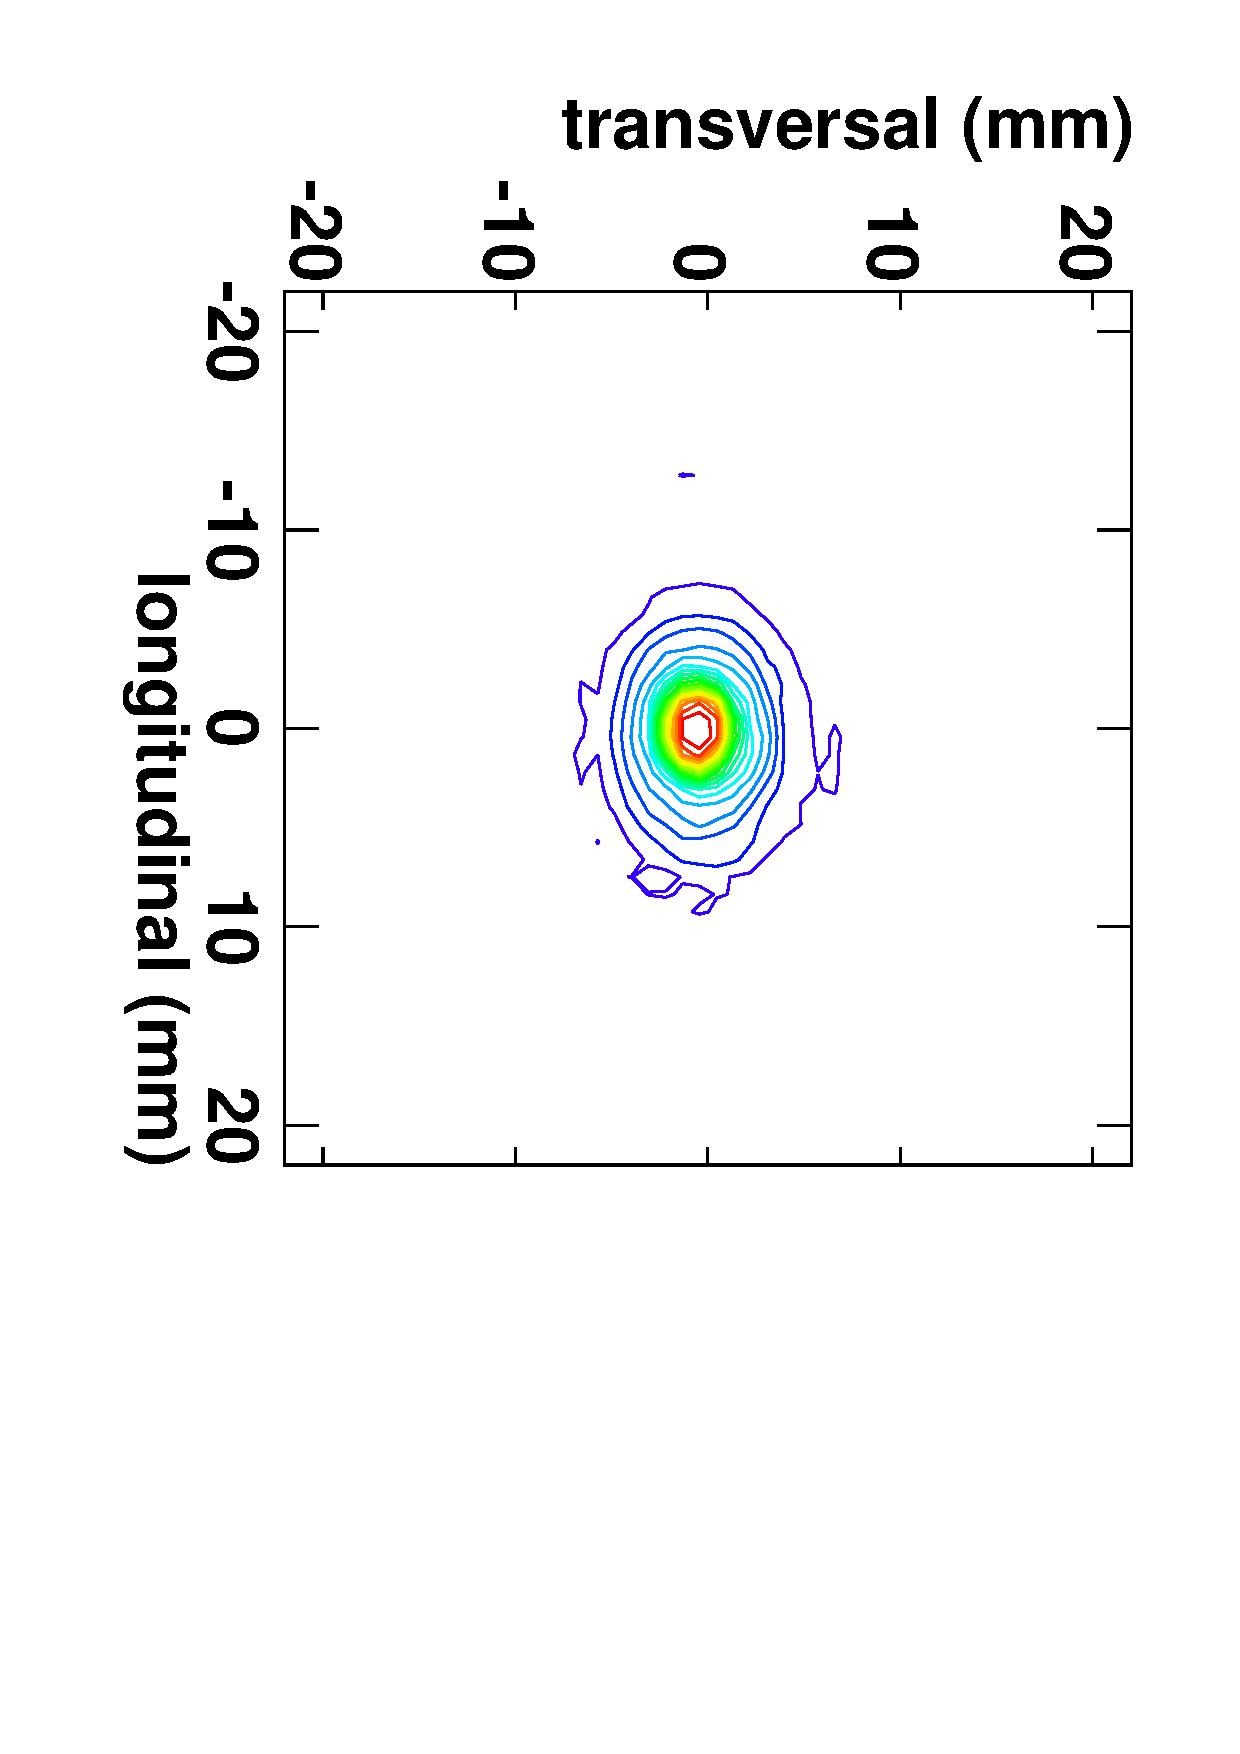
\includegraphics[angle=90,width=0.3\linewidth]{figures/Inj2/1mA40.pdf}\\
  I=1mA.Up: turn 0, 5, 10. Down: turn 20, 30, 40 by \opalcycl
}


\section{Conclusions}
\frame{
  \frametitle{Conclusions }
  \begin{block}{}
    \begin{enumerate}
    \item Establish a physical model which covers neighboring bunch effects self consistently
    \item Develop a 3D parallel PIC code \opalcycl, as a flavor of \opal
    \item Perform the first parallel simulation of multiple bunches in cyclotron
    \item Study neighboring bunch effects on the beam's evolution quantitatively on PSI Ring cyclotron
    \end{enumerate}
   \end{block}
}

\section{Acknowledgments}
\frame{
  \frametitle{Acknowledgments}
  \begin{block}{}
  \large{
    C. Kraus, T. Schietinger, W. Joho, S. Adam and AMAS group member,
    and those who have rendered support and help.}
  \end{block}
  \center { \Huge { *** } }
  \begin{block}{} 
    \center \Huge {Thanks for your attention!}
  \end{block}
}

\end{document}

